  % The main file for CAMP reports
 % Don't put any content in here. 
 % Don't even include content files by using \input or \inlcude. 
 % Put your content to TEXT.TEX or include it there using \input.
 % Uses:
 %		SETTINGS.TEX	contains the settings for this document
 %		COMMANDS.TEX	contains commands which can be used while writing
 %		INFO.TEX			contains the author, title and so on for the cover
 %		COVER.TEX			formats the front cover of the document
 %		ABSTRACT.TEX	contains the abstract to be included (if needed)
 %		TEXT.TEX			contains the actual content of the document
 %		BIB.BIB				containt the BibTeX entries for the document
 
 
%% Draft document mode
%% Final document
\documentclass[11pt,a4paper,bibtotoc,idxtotoc,headsepline,footsepline,footexclude,BCOR12mm,DIV13]{scrbook}

%\documentclass[11pt,a4paper,bibtotoc,idxtotoc,headsepline,footsepline,footexclude,BCOR20mm,DIV10]{scrbook}

% KOMA-Optionen:
%  bibtotoc: include bibliography in table of contents
%  idxtotoc: include index in table of contents
%  headsepline: use horizontalline under heading
%  BCOR: binding correcion (Bindungskorrektur) (e.g.: BCOR5mm)
%  DIV: Number of sheet sections (used for layout) (e.g.: DIV12) 



% include title and author information for the cover
% Set here the title, authors and other stuff to be used for the cover
% This file is used by MAIN.TEX

% set title, authors and stuff for the cover
\def\doctype{Master's Thesis}
\def\title{High-Dimensional Uncertainty Quantification of Fluid-Structure Interaction}
\def\titleGer{Hochdimensionalen Uncertainty Quantification der Fluid-Struktur-Interaktion}
\def\author{Ionut-Gabriel Farcas}
\def\date{}

% text to appear in the footer
\def\footertext{}

% include settings
% Included by MAIN.TEX
% Defines the settings for the CAMP report document

\renewcommand{\sectfont}{\normalfont \bfseries}        % Schriftart der Kopfzeile

% manipulate footer
\usepackage{scrpage2}
\pagestyle{scrheadings}
\ifoot[\footertext]{\footertext} % \footertext set in INFO.TEX
%\setkomafont{pagehead}{\normalfont\rmfamily}
\setkomafont{pagenumber}{\normalfont\rmfamily}

%% allow sophisticated control structures
\usepackage{ifthen}

% use Palatino as default font
\usepackage{palatino}

% enable special PostScript fonts
\usepackage{pifont}

\usepackage{dirtree}

% for inputing C++ code
\usepackage{listings}
\lstset { %
    language=C++,
    basicstyle=\footnotesize,% basic font setting
}

% make thumbnails
\usepackage{thumbpdf}

%to use the subfigures
%\usepackage{subfigure}
\usepackage{subfig}

\usepackage{colortbl}

% table
\usepackage{longtable}

%% show program code\ldots
%\usepackage{verbatim}
%\usepackage{program}

%% enable TUM symbols on title page
\usepackage{styles/tumlogo}

% for algorithms
\usepackage{algpseudocode,algorithm,algorithmicx}

\usepackage{multirow}

%% use colors
\usepackage{color}

%% make fancy math
\usepackage{amsmath}
\usepackage{amsfonts}
\usepackage{amssymb}
\usepackage{textcomp}
\usepackage{yhmath} % fr die adots 
%% mark text as preliminary
%\usepackage[draft,german,scrtime]{prelim2e}

%% create an index
\usepackage{makeidx}

% for the program environment
\usepackage{float}

%% load german babel package for german abstract
%\usepackage[german,american]{babel}
\usepackage[german,english]{babel}
\selectlanguage{english}

% use german characters as well
\usepackage[latin1]{inputenc}       % allow Latin1 characters

% use initals dropped caps - doesn't work with PDF
%\usepackage{dropping}
 %\usepackage[dvips]{dropping}

\usepackage{styles/shortoverview}
%----------------------------------------------------
%      Graphics and Hyperlinks
%----------------------------------------------------

%% check for pdfTeX
\ifx\pdftexversion\undefined
 %% use PostScript graphics
 \usepackage[dvips]{graphicx}

 \DeclareGraphicsExtensions{.eps,.epsi}
 \graphicspath{{figures/}{figures/review}} 
 %% allow rotations
 \usepackage{rotating}
 %% mark pages as draft copies
 %\usepackage[english,all,light]{draftcopy}
 %% use hypertex version of hyperref
 \usepackage[hypertex,hyperindex=false,colorlinks=false]{hyperref}
\else %% reduce output size \pdfcompresslevel=9
 %% declare pdfinfo
 %\pdfinfo { 
 %  /Title (my title) 
 %  /Creator (pdfLaTeX) 
 %  /Author (my name) 
 %  /Subject (my subject	) 
 %  /Keywords (my keywords)
 %}
 %% use pdf or jpg graphics
 \usepackage[pdftex]{graphicx}
 \DeclareGraphicsExtensions{.jpg,.JPG,.png,.pdf,.eps}
 \graphicspath{{figures/}} 
 
 %% Load float package, for enabling floating extensions
 \usepackage{float}
 
 %% allow rotations
 \usepackage{rotating}
 %% use pdftex version of hyperref
 \usepackage[pdftex,colorlinks=true,linkcolor=red,citecolor=red,%
 anchorcolor=red,urlcolor=red,bookmarks=true,%
 bookmarksopen=true,bookmarksopenlevel=0,plainpages=false%
 bookmarksnumbered=true,hyperindex=false,pdfstartview=%
 ]{hyperref}
%
%\usepackage[pdftex,colorlinks=false,linkcolor=red,citecolor=red,%
% anchorcolor=red,urlcolor=red,bookmarks=true,%
% bookmarksopen=true,bookmarksopenlevel=0,plainpages=false%
% bookmarksnumbered=true,hyperindex=false,pdfstartview=%
% ]{hyperref}
\fi




%% Fancy chapters
%\usepackage[Lenny]{fncychap}
%\usepackage[Glenn]{fncychap}
%\usepackage[Bjarne]{fncychap}

%\usepackage[avantgarde]{quotchap}

% set the bibliography style
%\bibliographystyle{styles/bauermaNum}
%\bibliographystyle{alpha}
\bibliographystyle{plain}

% include commands
% Commands to be used within the TUM report document
% Included by MAIN.TEX
% Please include your own cool commands here. 
% Be only sure to comment it sufficiently so others can use it.

%-------------------------------------------------------------
%                      Own Commands
%-------------------------------------------------------------


%-------------------------------------------------------------
% math stuff -------------------------------------------------

% nice R, N, C
\newcommand{\nat}{\mathbb{N}}
\newcommand{\real}{\mathbb{R}}
\newcommand{\compl}{\mathbb{C}}


\newcommand*\Let[2]{\State #1 $\gets$ #2}

\renewcommand*\Call[2]{\textproc{#1}(#2)}

% norm
\newcommand{\norm}[1]{\left\| #1 \right\|}

% un demi
\newcommand{\half}{\frac{1}{2}}

% parantheses
\newcommand{\parenth}[1]{ \left( #1 \right) }
\newcommand{\bracket}[1]{ \left[ #1 \right] }
\newcommand{\accolade}[1]{ \left\{ #1 \right\} }
%\newcommand{\angle}[1]{ \left\langle  #1 \right\rangle }

% partial derivative: %#1 function, #2 which variable
% simple / single line version
\newcommand{\pardevS}[2]{ \delta_{#1} f(#2) }
% fraction version
\newcommand{\pardevF}[2]{ \frac{\partial #1}{\partial #2} }

% render vectors: 3 and 4 dimensional
\newcommand{\veciii}[3]{\left[ \begin{array}[h]{c} #1 \\ #2 \\ #3	\end{array} \right]}
\newcommand{\veciv}[4]{\left[ \begin{array}[h]{c} #1 \\ #2 \\ #3 \\ #4	\end{array} \right]}

% render matrices: 3  dimensional (arguments in row first order)
\newcommand{\matiii}[9]{\left[ \begin{array}[h]{ccc} #1 & #2 & #3 \\ #4 & #5 & #6 \\ #7 & #8 & #9	\end{array} \right]}
%DOESN'T WORK,DON'T KNOW WHY \newcommand{\mativ}[16]{\left[ \begin{array}[h]{cccc} #1 & #2 & #3 & #4 \\ #5 & #6 & #7 & #8 \\ #9 & #10 & #11 & #12 \\ #13 & #14 & #15 & #16 \end{array} \right]}


%-------------------------------------------------------------
%-------------------------------------------------------------


%-------------------------------------------------------------
% some abreviations ------------------------------------------
\newcommand{\Reg}{$^{\textregistered}$}
\newcommand{\reg}{$^{\textregistered}$ }
\newcommand{\Tm}{\texttrademark}
\newcommand{\tm}{\texttrademark~}
\newcommand {\bsl} {$\backslash$}

%-------------------------------------------------------------
%-------------------------------------------------------------


%-------------------------------------------------------------
% formating --------------------------------------------------

% Theorem & Co environments and counters
\newtheorem{theorem}{Theorem}[chapter]
\newtheorem{lemma}[theorem]{Lemma}
\newtheorem{corollary}[theorem]{Corollary}
\newtheorem{remark}[theorem]{Remark}
\newtheorem{definition}[theorem]{Definition}
\newtheorem{equat}[theorem]{Equation}
\newtheorem{example}[theorem]{Example}
%\newtheorem{algorithm}[theorem]{Algorithm}

% inserting figures
\newcommand{\insertfigure}[4]{ % Filename, Caption, Label, Width percent of textwidth
	\begin{figure}[htbp]
		\begin{center}
			\includegraphics[width=#4\textwidth]{#1}
		\end{center}
		\vspace{-0.4cm}
		\caption{#2}
		\label{#3}
	\end{figure}
}


%%%%%%%%%%%%%%%%%%%% Referencing commands %%%%%%%%%%%%%%%%%%

% referencing figures
\newcommand{\refFigure}[1]{ %label
	figure \ref{#1}
}

% referencing chapters
\newcommand{\refChapter}[1]{ %label
	chapter \ref{#1}
}

%referencing sections
\newcommand{\refSection}[1]{ %label
	section \ref{#1}
}

%referencing paragraphs
\newcommand{\refParagraph}[1]{ %label
	paragraph \ref{#1}
}

%referecing equations
\newcommand{\refEquation}[1]{ %label
	equation \ref{#1}
}

%referecing tables
\newcommand{\refTable}[1]{ %label
	table \ref{#1}
}

%%%%%%%%%%%%%%%%%%%%%%%%%%%%%%%%%%%%%%%%%%%%%%%%%%%%%%%%%%%%%%%%%%%

\newcommand{\rigidTransform}[2]
{
	${}^{#2}\!\mathbf{H}_{#1}$
}

%code, in typewriter
\newcommand{\code}[1]
 {\texttt{#1}}

% comment that appears on the border - very practical !!!
\newcommand{\comment}[1]{\marginpar{\raggedright \noindent \footnotesize {\sl #1} }}

% page clearing
\newcommand{\clearemptydoublepage}{%
  \ifthenelse{\boolean{@twoside}}{\newpage{\pagestyle{empty}\cleardoublepage}}%
  {\clearpage}}


%-------------------------------------------------------------
%-------------------------------------------------------------


\newcommand{\etAl}{\emph{et al.}\mbox{ }}


\makeindex
	%% inter line spacing
%\linespread{1.0}

\makeglossary

\begin{document}

	\frontmatter
	
	
	%% The front cover for the TUM report document.
% Included by MAIN.TEX


%--------------------------------------------------
% The Front Cover
%--------------------------------------------------

% The front cover for the TUM document.
% Included by MAIN.TEX


%--------------------------------------------------
% The Front Cover
%--------------------------------------------------

% correct BCOR - undo at the end !!!
\def\bcorcor{0.15cm}
\addtolength{\hoffset}{\bcorcor}

\thispagestyle{empty}

 \vspace{4cm}
\begin{center}
	       %\oTUM{4cm}
	       
	  
\includegraphics[width=4cm]{styles/tum_logo.png}
	   
	   \vspace{5mm}     
	   \huge Computational Science and Engineering \\(Int. Master's Program)\\ 
	   \vspace{0.5cm}
	 \large Technische Universit{\"a}t M{\"u}nchen\\
    \vspace{1mm}
        
	\end{center}
		

\vspace{15mm}
\begin{center}

   {\Large \doctype}

  \vspace{20mm}
  
  {\huge\bf \title}\\%[3ex]
  
  
  \vspace{15mm}
  
  
  {\LARGE  \author}
  
  \vspace{10mm}
  
  \begin{figure}[h!]
  \centering
   
\includegraphics[width=4cm]{styles/cse_logo.jpg}
  \end{figure}
  
  \end{center}
	\clearemptydoublepage
%	
%	% The titlepage for the CAMP report document.
% Included by MAIN.TEX


%--------------------------------------------------
% The title page
%--------------------------------------------------

% correct BCOR - undo at the end !!!
\def\bcorcor{0.15cm}
\addtolength{\hoffset}{\bcorcor}

\thispagestyle{empty}

 \vspace{10mm}
\begin{center}
	       %\oTUM{4cm}
	       
\includegraphics[width=4cm]{styles/tum_logo.png}
	   
	   \vspace{5mm}     
	   \huge Computational Science and Engineering \\(Int. Master's Program)\\ 
	   \vspace{0.5cm}
	 \large Technische Universit{\"a}t M{\"u}nchen\\
        
	\end{center}
		

\vspace{10mm}
\begin{center}

   {\Large \doctype}

  \vspace{10mm}
  
  {\LARGE \title}\\
  
  
  \vspace{10mm}
  
  
  {\LARGE  \titleGer}\\
  
  
  \vspace{10mm}

    %\hfill
    \begin{tabular}{ll}
	   \Large Author:     & \Large \author \\[2mm]
	   \Large $\mathrm{1^{st}}$ examiner:    & \Large Prof. Dr. Hans-Joachim Bungartz \\[2mm]				
	   \Large $\mathrm{2^{nd}}$ examiner:    & \Large Prof. Dr. rer. nat. habil. Miriam Mehl \\[2mm]
	   \Large Assistant advisor:    & \Large Dipl.-Math. Benjamin Uekermann \\[2mm]
	   \Large Thesis handed in on:       & \Large We'll see when, 2015
	 \end{tabular}
	 
	 \vspace{5mm}
	 
	 \begin{figure}[h!]
  \centering
   
\includegraphics[width=4cm]{styles/cse_logo.jpg}
  \end{figure}
   

\end{center}

% undo BCOR correction
\addtolength{\hoffset}{\bcorcor}
	
	
%	\input{components/cover_maschmeyer}
	%\clearemptydoublepage
	
	%% The titlepage for the CAMP report document.
% Included by MAIN.TEX


%--------------------------------------------------
% The title page
%--------------------------------------------------

% correct BCOR - undo at the end !!!
\def\bcorcor{0.15cm}
\addtolength{\hoffset}{\bcorcor}

\thispagestyle{empty}

 \vspace{10mm}
\begin{center}
	       %\oTUM{4cm}
	       
\includegraphics[width=4cm]{styles/tum_logo.png}
	   
	   \vspace{5mm}     
	   \huge Computational Science and Engineering \\(Int. Master's Program)\\ 
	   \vspace{0.5cm}
	 \large Technische Universit{\"a}t M{\"u}nchen\\
        
	\end{center}
		

\vspace{10mm}
\begin{center}

   {\Large \doctype}

  \vspace{10mm}
  
  {\LARGE \title}\\
  
  
  \vspace{10mm}
  
  
  {\LARGE  \titleGer}\\
  
  
  \vspace{10mm}

    %\hfill
    \begin{tabular}{ll}
	   \Large Author:     & \Large \author \\[2mm]
	   \Large $\mathrm{1^{st}}$ examiner:    & \Large Prof. Dr. Hans-Joachim Bungartz \\[2mm]				
	   \Large $\mathrm{2^{nd}}$ examiner:    & \Large Prof. Dr. rer. nat. habil. Miriam Mehl \\[2mm]
	   \Large Assistant advisor:    & \Large Dipl.-Math. Benjamin Uekermann \\[2mm]
	   \Large Thesis handed in on:       & \Large We'll see when, 2015
	 \end{tabular}
	 
	 \vspace{5mm}
	 
	 \begin{figure}[h!]
  \centering
   
\includegraphics[width=4cm]{styles/cse_logo.jpg}
  \end{figure}
   

\end{center}

% undo BCOR correction
\addtolength{\hoffset}{\bcorcor}
	
	
	%\clearemptydoublepage


\thispagestyle{empty}
\selectlanguage{english}
	\vspace*{0.8\textheight}
	\noindent
	I hereby declare that this thesis is entirely the result of my own work except where otherwise indicated. I have only used the resources given in the list of references.
	
	\vspace{15mm}
	\noindent
	\today \hspace{5cm} \author
\selectlanguage{english}
\newpage
	
	%\clearemptydoublepage
\phantomsection
\addcontentsline{toc}{chapter}{Acknowledgements}	


%\chapter*{Acknowledgements}

\vspace*{2cm}

\begin{center}
{\Large \bf Acknowledgments}
\end{center}

\vspace{1cm}




	%
	%% Abstract for the TUM report document
% Included by MAIN.TEX


\clearemptydoublepage
\phantomsection
\addcontentsline{toc}{chapter}{Abstract}	





\vspace*{2cm}
\begin{center}
{\Large \bf Abstract}
\end{center}
\vspace{1cm}

	\textit{Fluid-Structure Interaction} (FSI) problems, where one or more structures interact with an internal or surrounding fluid flow, play prominent role in many scientific fields, that pose many challenges do to their strong non-linearity and multidisciplinary nature. Some of the most important challenges in FSI are \textit{multi-domain} character and \textit{interface coupling conditions}, combining \textit{different coordinate systems}, \textit{designing robust and efficient numerical methods} that ideally provide optimal convergence order and demand for \textit{high performance computing}, making FSI a complex domain by itself. Furthermore, \textit{uncertainty}, which appears naturally in most problems (\textit{e.g in density of fluid or/and material, viscosity of the fluid, etc}) is another challenge in FSI. This is modelled by \textit{Uncertainty Quantification} (UQ). One of the most important challenges in UQ is the \textit{multidimensional} stochastic problems. The classical approaches are \textit{computationally expensive} and are usually infeasible for more than few dimensions. In order to tackle these \textit{multi-challenges), one needs to use \textit{sophisticated mathematical methods} and \textit{high performance computing}.
	
	The aforementioned challenges constitute the motivation precursor for this thesis; using \textit{forward-propagation} of the uncertainty in input parameters, the aim is to \textit{investigate the uncertainty in FSI problems}, via \textit{sophisticated mathematical methods} and \textit{high performance computing} (multi-core architectures and parallel algorithms). In more details, \textit{non-intrusive} methods based on \textit{sampling} will be used. These methods are \textit{Monte Carlo sampling} (MCS) and \textit{Stochastic Collocations} (SC), that is based on \textit{generalized Polynomial Chaos} (gPC) methodology. While MCS uses multiple samples generated based on a prescribed \textit{probability density function} (pdf) which serve as input in the underlying deterministic numerical algorithm, SC approximates the solution on a prescribed set of points, called \textit{nodes}, which serve as collocations points. From this approximation, useful information (\textit{e.g. statistics}) can be easily extracted. Since for each \textit{sample} or \textit{node}, the numerical problems are \textit{independent} in both methods, these schemes are \textit{embarrassingly parallel}, hence suitable for high performance computing. One of the major differences between them is the \textit{convergence rate}; while the convergence rate is very slow for MCS, the one of SC is \textit{exponential in n} for suitable input pdfs. Due to the complex nature of FSI, the UQ methodology will be implemented on certain \textit{model FSI problems}.
	
	Lastly, \textit{multi-dimensional} stochastic problems are also being considered. Whereas MCS is independent of the dimensionality (and of the input pdf), in SC, in which numerical quadrature is employed, the \textit{curse of dimensionality} occurs. In order to overcome it, \textit{sparse grids} will be employed and to this extent, the SG++ library is to be used. 

	\tableofcontents
  
  %\clearemptydoublepage

\phantomsection
\addcontentsline{toc}{chapter}{Outline of the Thesis}

\begin{center}
	\huge{Outline of the Thesis}
\end{center}




%--------------------------------------------------------------------
\section*{Part I: Introduction and Theory}

\noindent {\scshape Chapter 1: Introduction}  \vspace{1mm}

\noindent  This chapter presents an overview of the thesis and it purpose. Furthermore, it will discuss the sense of life in a very general approach.  \\

\noindent {\scshape Chapter 2: Theory}  \vspace{1mm}

\noindent  No thesis without theory.   \\

%--------------------------------------------------------------------
\section*{Part II: The Real Work}

\noindent {\scshape Chapter 3: Overview}  \vspace{1mm}

\noindent  This chapter presents the requirements for the process.

	\mainmatter
	
	
		% ---------------------------------------------------------------------------
		%
		% Introduction and Background Theory
		%
		% ---------------------------------------------------------------------------
		\chapter{Introduction}
\label{chapter:Introduction}
\begin{itemize}
\item Some words about FSI and UQ
\item Example applications
\item Challenges in FSI and UQ; motivation for HPC and sophisticated mathematics
\item ...
\end{itemize}	
\section{Problem Statement}
\label{sec:Problem Statement}
\begin{itemize}
\item Project Context
\item Perspective from different points of views: practical, HPC, multi-challenge?
\item Aims and challenges
\item Desired outcomes
\item ...
\end{itemize}	
\section{The Multi-Challenge}
\label{sec:The Multi-Challenge}
\begin{itemize}
\item What is the multi-challenge
\item Multi-physics and multi-domain FSI + multi-dimensional uncertainty
\item Challenges within the multi-challenge
\item ...
\end{itemize}	
\section{Related Work}
\label{sec:Related Work}
\begin{itemize}
\item Relevant work that was done for FSI + UQ
\item ...
\end{itemize}
And then motivate the structure and to what each chapter focuses on



		% ---------------------------------------------------------------------------
		%
		% Fluid-Structure Interaction Introduction
		%
		% ---------------------------------------------------------------------------
		\chapter{Fluid-Structure Interaction}
\label{chapter:Fluid-Structure Interaction}
	This chapter aims to provide an overview of the \emph{Fluid-Structure Interaction} (FSI) segment of this work. The first two sections brief the \emph{theoretical} (\refSection{sec:Theoretical Background}) and \emph{modelling} (\refSection{sec:Modelling}) aspects of FSI, used within this work, such as the \emph{multi-physics} aspect of FSI, mathematical description of fluids and structures, as well as the approaches used for solving an FSI problem. The last two sections are destined to overview the employed \emph{FSI codes}, i.e. the multi-physics package \emph{Alya} and the coupling library \emph{preCICE}.
\section{Theoretical Background}
\label{sec:Theoretical Background}
\begin{itemize}
\item A few words about fluid mechanics and solid mechanics
\item Multi-physics
\item Lagrangian and Eulerian perspectives ; motivation for ALE
\item Some FSI literature review
\item ...
\end{itemize}
\section{Modelling}
\label{sec:Modelling}
\begin{itemize}
\item State Reynold Transport theorem
\item State incompressible Navier-Stokes equations + constitutive equations 
\item State solid modelling + constitutive equations
\item partitioned vs. monolithic approach
\item ...
\end{itemize}	
\section{General Description of the Multi-Physics Code}
\label{sec:General Description of the Multi-Physics Code}
\begin{itemize}
\item Overview of Alya: what is it, what was designed for, etc
\item Important features
\item ...
\end{itemize}		
\section{General Description of the Coupling Library}
\label{sec:General Description of the Coupling Library}
\begin{itemize}
\item Overview of preCICE: what is it, what was designed for, etc
\item Important features
\item ...
\end{itemize}	
		% ---------------------------------------------------------------------------
		%
		% Forward propagation of uncertainty introduction
		%
		% ---------------------------------------------------------------------------
		\chapter{Forward Propagation of Uncertainty}
\label{chapter:Forward Propagation of Uncertainty}
\begin{itemize}
\item Brief summary of what the chapter will contain
\end{itemize}
\section{Theoretical Background}
\label{sec:Theoretical Background}
\begin{itemize}
\item Explain what is forward propagation of uncertainty
\item What is assumed to be known
\item ..
\end{itemize}
\section{Probabilistic Modelling}
\label{sec:Probabilistic Modelling}
\begin{itemize}
\item Introduce a generic probabilistic space, where the stochastic modelling is made
\item Reminder of what are univariate and multivariate random variables
\item Important: we work only with iid random vars; plus what this implies
\item Formulas for expectation and variance for one dim and multi dim rand vars
\item ...
\end{itemize}	
\section{Overview of Sampling Methods}
\label{sec:Overview of Sampling Methods}
\begin{itemize}
\item Brief reminder of what sampling methods are and specify some examples
\item Explain polynomial and generalized polynomial chaos methodology (from Wiener until Xiu and collaborators)
\item Why to use gPC (e.g. because of the advancements in HPC, etc)
\item Literature review
\item ...
\end{itemize}	
\section{Monte Carlo Sampling}
\label{sec:Monte Carlo Sampling}
\begin{itemize}
\item Overview of Monte Carlo methodology in the UQ context
\item ...
\end{itemize}	
\subsection{One-Dimensional Case}
\label{subsec:One-Dimensional Case}
\begin{itemize}
\item Describe the algorithm in a one-dimensional stochastic setting
\item ...
\end{itemize}	
\subsection{Multi-Dimensional Case}
\label{subsec:Multi-Dimensional Case}
\begin{itemize}
\item Describe the algorithm in a multi-dimensional stochastic setting
\item ...
\end{itemize}
\subsection{Convergence Analysis and Properties}
\label{subsec:Convergence Analysis and Properties}
\begin{itemize}
\item Properties: e.g. Convergence for generic Monte Carlo sampling + ways to improve it (e.g. quasi Monte Carlo), independence of dimension, distribution, parallelization, numerical errors, etc
\item Pros and Cons; Motivate Collocations
\end{itemize}	
\section{Stochastic Collocations}
\label{sec:Stochastic Collocations}
\begin{itemize}
\item Briefly explain what collocations are
\item Specify that MCS is just a particular case of collocations, using the delta function as stochastic basis
\item ...
\end{itemize}
\subsection{Pseudo-spectral Approach}
\label{subsec:Gaussian Quadrature}
\begin{itemize}
\item Describe what does the pseudo-spectral approach look like and that is based on quadrature
\item Explain Gauss based quadrature: Gauss-Hermite and Gauss-Legendre
\item Explain how to compute the statistics with this approach
\item Explain the restrictions imposed to the mean and standard deviation of the random variable $(\sqrt{2}*node*stddev + mean > 0 => mean/stddev > - \sqrt{2}*node!)$
\item ...
\end{itemize}	
\subsection{One-Dimensional Case}
\label{subsec:One-Dimensional Case}
\begin{itemize}
\item Describe the algorithm in a one-dimensional stochastic setting
\item ..
\end{itemize}	
\subsection{Multi-Dimensional Case}
\label{subsec:Multi-Dimensional Case}
\begin{itemize}
\item Describe the algorithm in a multi-dimensional stochastic setting
\item Curse of dimensionality with brute force approach
\item ..
\end{itemize}
\subsection{Convergence Analysis and Properties}
\label{subsec:Convergence Analysis and Properties}
\begin{itemize}
\item Properties: convergence (exponential also outside the Askey scheme!!), parallelization, non-intrusive, dependence on distribution and dim, numerical errors, etc
\item Pros and Cons of the method 
\item ...
\end{itemize}	
\section{Sparse Grids Stochastic Collocations}
\label{sec:Sparse Grids Stochastic Collocations}
\begin{itemize}
\item Brief overview of SG-SCS
\item A way to (partially) break the curse of dimensionality
\item ...
\end{itemize}
\subsection{Overview of Sparse Grids}
\label{subsec:Overview of Sparse Grids}
\begin{itemize}
\item Overview of sparse grid methodology
\item Quadrature on sparse grids
\item ...
\end{itemize}	
\subsection{Sparse Grids Toolbox SG++}
\label{subsec:Sparse Grids Toolbox SG++}
\begin{itemize}
\item Brief overview of SG++ and its capabilities
\item Explain how quadrature works within SG++
\item Improvements gained from using SG++ (no of collocation points, memory, convergence, etc)
\item ...
\end{itemize}
\section{Probability Density Function Estimation}
\label{sec:Probability Density Function Estimation}
\subsection{General Description}
\label{subsec:General Description}
\begin{itemize}
\item Overview of what density estimation is and why we use it here
\item Some methods: brute force, KDE, etc
\item ...
\end{itemize}
\subsection{Kernel Density Estimation}
\label{subsec:Kernel Density Estimation}
\begin{itemize}
\item Explain what KDE is
\item Examples of Kernels
\item Implementation using Python scikit toolbox
\item ...
\end{itemize}
		% ---------------------------------------------------------------------------
		%
		% Details regarding the implementation
		%
		% ---------------------------------------------------------------------------
		\chapter{Implementation Details}
\label{chapter:Implementation Details}
	The purpose of this chapter is to present the implemented UQ software and it is divided into four sections. A general description is given in the first section, providing a general overview of the implementation, its functionality and properties, as well as how its interaction with the application code. The next three sections present o more detailed description, focusing on the implementation's constitutive modules: \emph{pre-processing} phase, described in \refSection{sec:Pre-processing}, UQ \emph{simulation} phase, described in \refSection{sec:Simulation} and at the end, the \emph{post-processing} step, described in \refSection{sec:Post-processing}.
\section{General Description}
\label{sec:General Description}
	The UQ software consists of a main \emph{C++ implementation} together with a set of external \emph{tools} used for interacting with the application code. One of its important features is its \emph{non-intrusive interaction} with the FSI software, by only needing access to the \emph{configuration} files and the \emph{executable} file of the multi-physics software, hence, treating the FSI solver as a \emph{black box}. Furthermore, its \emph{configuration} is done via a text file, at \emph{runtime}, facilitating e.g. the switch between UQ methods or probability distributions, without the need for recompiling the code. The configuration step is further explained in the following paragraph. Another key feature is comprised by the division into \emph{three main modules}, i.e. \emph{pre-processing}, \emph{simulation} and \emph{post-processing}, which  provides an easier understanding of the code, facilitates its easier extension and/or improvement and also permits its usage as a library\footnote{for the moment, this only works for applications codes with a structure similar to the ones used in this work}. Last but not least, although the code was tested for only two specific applications, it can be easily altered to work for any application similar to the ones considered in this work, whose configuration is done via \emph{external files}, with the alteration being done for the tools used to interact with the application code.
	
	It should be noted that the location of the UQ code is assumed to be \emph{test case/uq code}, thus, all tools that interact with the application code require a relative path to the it. Moreover, the configuration file is located inside \emph{uq code/}. It is a \emph{text file} named \emph{configuration.uq} that obeys the following editing rules:
\begin{itemize}
\item lines that start with $\#$ are ignored
\item configuration lines are of the form: \emph{name} = \emph{value}
\item no line is allowed to be empty
\end{itemize}
	This implies that a line of this file has the form e.g. \emph{nsamples = 100}. It is comprised of three main parts, each responsible for a certain type of configuration.
\begin{enumerate}
\item communication with the application code configuration \newline
In this part, the \emph{relative path} to the external tools and specific application code files is given. As an example, the set-up for the relative path to the tool used to modify the \emph{viscosity} value for the fluid is: \emph{insert$\_$nastin$\_$exec = ../tools/util/insert$\_$params$\_$nastin$\_$vis}. 
\item UQ problem configuration \newline
In this segment, the user can set-up UQ specific data, such as which \emph{algorithm} to employ, which \emph{pdf} to use in order to model the input uncertainty, the number of samples for Monte Carlo Sampling, the \emph{quadrature degree} for Stochastic Collocations, etc. Although is not a hard restriction, it is preferred that the \emph{algorithm} and \emph{pdf} are specified as \emph{boolean} variables, with the following convention: 0 for Monte Carlo, 1 for Collocations and 0 for normal distribution and 1 for uniform distribution, respectively. As an example, the set-up for normal distribution is \emph{pdf = 0}. If this rule is not met, an error message is output on the console.
\item stochastic problem set-up \newline
In the final part, the numerical values for the \emph{two parameters} characterizing the uncertain input(s) are specified; for \emph{normal} distribution, the parameters are the \emph{mean} and the \emph{standard deviation}, whereas for \emph{uniform} distribution, the \emph{left} and \emph{right} interval boundaries, respectively. As an example, if the fluid density is modelled as a normal random variable, its configuration is \emph{rho$\_$f$\_$p1 = 0.01}, followed by  \emph{rho$\_$f$\_$p2 = 0.001}.
\end{enumerate}
		
	The C++ implementation consists of a sequence of \emph{classes} having the functionality outlined in the \emph{sampling algorithms}, described in \refChapter{chapter:Forward Propagation of Uncertainty}, together with their additional required capabilities. This means that for \emph{Monte Carlo Sampling}, classes used to elicit a \emph{user defined} number of \emph{normal}  and \emph{uniform random variables} are implemented, while for \emph{Stochastic Collocations}, the additional required functionality consists of classes that generate \emph{nodes} and \emph{weights} used for numerical quadrature. Moreover, additional functions are implemented in a separate helper library, used to e.g. parse the configuration file, create strings with user defined names used to call external tools, etc. An important remark is that the external tools, as well as the multi-physics software's executable file are called via \emph{system} calls\footnote{the \emph{int system (const char* command)} function is available in the \emph{cstdlib} C++ library}. 
		
	The end of the implementation process resulted in \emph{six projects}, with the following capabilities: the first three \emph{serial} UQ implementations consist in one for a \emph{one-dimensional} problem, one for a scenario with \emph{two stochastic dimensions} and one for a \emph{multi-dimensional} stochastic problem. These codes are built as \emph{one stand-alone applications}, with integrated constitutive modules.  Although they encompass the entire UQ simulation pipeline, they proved to be of little use for the testing phase because of the \emph{complexity} of the simulated scenarios. Even if the application codes are already parallel, together with the reduced combined cost of the pre-processing and post-processing phase compared to the simulation cost, a \emph{serial}\footnote{in this context, \emph{serial} means either a completely serial application or one that is serial, except for the application code} is not practically feasible. Moreover, it also contradicts one of the goals of this work, the use of \emph{HPC}. Given these, the next logical step seemed to be the \emph{transformation} of the serial implementations into parallel ones, more specifically, \emph{process (MPI-based) parallel} and hence, obtaining an HPC suited application. This was not possible, given the reasons mentioned in \refSection{sec:General Description of the Multi-Physics Code} and \refSection{sec:General Description of the Coupling Library}: the used application code already uses MPI, thus, it is not possible to use MPI in the UQ code as well. This restriction gave rise to two possibilities: either \emph{compile} the application code so that it does not use MPI, i.e. compile preCICE with \emph{mpi=off} flag and Alya with \emph{make}, or \emph{decouple} the UQ code so that the three constitutive modules are separated, opening the possibility to run the \emph{simulation} module in a \emph{pseudo-parallel fashion}, by taking advantage of the \emph{MAC Cluster's batch system} capabilities. Taking once again into account the complexity and the high compute and memory requirements of the tested scenarios, the \emph{second} option was adopted in this work. The decoupled approach can be summarized as follows: after the pre-processing is performed for a user defined number of UQ points\footnote{either samples, for Monte Carlo sampling, or quadrature nodes, for Stochastic Collocations}, the simulation part is done via launching \emph{simultaneously} an equal number of \emph{batch scripts}, letting the cluster's batch system to administrate their run, depending on the degree of cluster's occupancy. Finally, after all simulations are performed, the post-processing phase is realized. This is further explained in the next three sections. In the following paragraph, an overview of all presented implementations is provided.
	
	The motivation behind designing a one-dimensional stochastic implementation stems from the fact that before any multi-dimensional simulation is performed, the one-dimensional ones are to be performed in order to understand \emph{how} does the uncertainty in the input physical parameters affect the underlying simulation scenario and based on the obtained results, to formulate \emph{relevant multi-dimensional} scenarios. The two-dimensional code differs from a \emph{generic multi-dimensioanl} one by the fact that the implementation for Stochastic Collocations is realized using \emph{brute-force}, i.e. the two-dimensional quadrature is done using a \emph{tensor product} basis of the one-dimensional case. This means that for, e.g. Gauss-Hermite quadrature, one has (add reference!):
\begin{equation} \label{eq:2dimquad}
\int_\real{\int_\real{f(x,y)dxdy}} = \sum_{i=0}^n{\sum_{j=0}^n{f(\zeta_i, \zeta_j)\omega_i \omega_j}},
\end{equation}
where $\zeta_i, \omega_i, \zeta_j, \omega_j, i=0\ldots n, j=0\ldots n$ are the pair of \emph{nodes} and respectively the \emph{weights} for each dimension. This implementation serves as a comparison tool against the SG++ based implementation because of the relatively similar required computational resources by both approaches, which is be further presented in \refChapter{chapter:Test Scenarios and Results}. Finally, the multi-dimensional\footnote{in this context, multi-dimensional implies dimension greater or equal to two} design aims to tackle an \emph{arbitrary dimensional} stochastic problem, featuring a multi-dimensional Sparse Grids Stochastic Collocations implementation and a multi-dimensional Monte Carlo sampling algorithm. 

	The use of C++ as the development language offered multiple advantages, including the possibility to create an implementation that is not only suited for \emph{HPC}, but also permits the usage of modern programming paradigms, such as \emph{object-oriented} programming. 
\dirtree{%
.1 main source file.
.2 UQ simulation.
.3 Monte Carlo simulation - normal distribution.
.3 Monte Carlo simulation - uniform distribution.
.4 Random number generator.
.5 Normal random variables.
.5 Uniform random variables.
.3 Stochastic Collocations simulation - normal distribution.
.3 Stochastic Collocations simulation - uniform distribution.
.4 Gaussian quadrature.
.5 Gaussian-Hermite quadrature.
.5 Gaussian-Legendre quadrature.
}
	At a conceptual level, the above diagram describes the UQ code structure as \emph{tree}, having the \emph{main source file} as root. The additional library containing the \emph{helper} functions was omitted, because it is not illustrative for the object oriented structure. As it can be inferred from the diagram, three \emph{parent} classes were used, each outlining a \emph{generic behaviour}: bottom-up, \emph{Gaussian quadrature} specifies the necessary states and behaviours for specific instances of Gaussian-based quadrature, needed by Stochastic Collocations. In the same fashion, the \emph{Random number generator} characterizes the functionality utilized by the specific random number generators used by Monte Carlo Sampling. Finally, a generic \emph{UQ simulation} class was defined, which outlines the generic, modular behaviour of the form pre-processing, simulation, post-processing.

	As it was already stated, the UQ implementation was designed to interact with the multi-physics code in a non-intrusive way. It needs access only to the \emph{configuration} files for the \emph{fluid} and \emph{structure} solvers. As an example, for the \emph{Vertical Flap} (c.f. \refSection{sec:Vertical Flap}), the configuration files are \emph{Flap.nsi.dat}- for the fluid solver and \emph{Flap.sld.dat}- for the structure solver. For the deterministic problem, the part where the physical parameters are set is:
\\
...
\\
 PROPERTIES \\
         DENSITY=    0.01 \\
         VISCOSITY=  0.03 \\
 END$\_$PROPERTIES \\
 ... \\
for the fluid solver and
\\
...
\\
 PROPERTIES \\
        DENSITY=             0.01 \\
  		CONSTITUTIVE$\_$MODEL   ISOLIN  0.5e5  0.3 \\
 END$\_$PROPERTIES \\
 ... \\
for the structure problem, where, the numbers from the CONSTITUTIVE$\_$MODEL line represent the \emph{Young's modulus} and \emph{Poisson's ratio}, respectively. It is important to emphasize that every Alya-based test case has two configuration files for the fluid and structure problem, respectively, of the form \emph{Name.nsi.dat} and \emph{Name.sld.dat}, where \emph{Name} is the conventional name of the test case. 
\newline

	In the following sections, the pre-processing, simulation and post-processing steps are explained in more detail. Because of the identical functionality provided by the \emph{serial} and \emph{de-serialized} implementations, each phase is similar for both types implementations. However, as the \emph{de-serialized} version was mainly used throughout simulations, in the following the emphasis is on solely on it.
\section{Pre-processing}
\label{sec:Pre-processing} 
	
	In the \emph{pre-processing} phase consists in set-up of the UQ problem. It differs for Monte Carlo Sampling and Stochastic Collocations, hence it is presented separately. However, given the \emph{robustness} of the Monte Carlo algorithm, the pre-processing step for \emph{one} or \emph{multi-dimensions} is \emph{almost identical}, as the only change from one to many dimensions is reflected by \emph{how many} random variables are to be generated. On the other hand, given the \emph{classical} and \emph{sparse grids} based implementations for Stochastic Collocations, the pre-processing phase differs and thus, it is presented distinctively, for both possibilities. As an observation, it is important to outline that before any simulation is done, it is assumed that the configuration is already set-up in \emph{configuration.uq}.
\newline
\textbf{Monte Carlo Sampling}
\newline
	For Monte Carlo Sampling, the first step is to generate a \emph{user-defined number of random variables}, depending on \emph{dimensionality}. This is realized using one of C++ standard library's pseudo-random number generators\footnote{all specific functions are available in \emph{random} library}, based on the \emph{Mersenne Twister 19937 generator} (add reference!) and the \emph{random device}, used as a \text{seed}, which provides a highly accurate way of generating random variables (add reference). This functionality is provided by classes \emph{NormalRandomVariable} and \emph{UniformRandomVariable}. Afterwards, via calling an external bash script tool called \emph{create$\_$data$\_$point}, a folder called simulation$\_i, i = 0...nsamples-1$ is created, corresponding to \emph{each} sample that contains \emph{two folders and one file}: \emph{nastin$\_i$} and \emph{solidz$\_i$}, $i = 0...nsamples-1$ and the \emph{preCICE configuration file} (c.f. \refSection{sec:General Description of the Coupling Library} ), respectively. In the \emph{nastin} and \emph{solidz} folders, the data that is needed by the multi-physics application code for one simulation is copied by the tool from \emph{a generic, deterministic set-up}. Succeeding the creation of the simulation folder is the \emph{replacement} of the deterministic physical parameter that was considered to be uncertain by the corresponding random variable. This is realized by calling an external Perl tool, with a name of the form \emph{insert$\_$params$\_$nastin$\_$} -for a fluid specific parameter, or \emph{solidz$\_$} - for a structure specific parameter, followed by the name of the parameter to be replaced. This tool edits the data file \emph{in-place}. All steps can be summarized in the following algorithm:
\begin{algorithm}
\caption{Pre-processing for arbitrary dimension Monte Carlo Sampling
\label{alg:1DMCS_preproc}}
  \begin{algorithmic}[1]
    \Require{$dimension$, $nsamples$ values \Comment{defined in the configuration file}}
    \For{$i \gets 0 \textrm{ to } dimension-1$}
    		\State call function that creates $nsamples$ random variables
    	\EndFor
    \For{$i \gets 0 \textrm{ to } nsample-1$}
        \State call create$\_$data$\_$point \Comment{create simulation$\_i$ folder}
        \State call insert$\_$new$\_$data \Comment{replace the underlying physical parameter in simulation$\_i$}
    \EndFor
  \end{algorithmic}
\end{algorithm}
\newline	
\textbf{Stochastic Collocations}
\newline
	As a general outline, the pre-processing phase for Stochastic Collocations can be summarized as following: depending on dimension, \emph{generate collocations points} - nodes and weight for classical approach, nodes for sparse grids approach - then \emph{create} \emph{simulation} folders, based on the number of collocation points and in the end, modify the underlying parameters that are considered to be uncertain in the solver's data files. In the following, these steps are put into perspective for each approach.
\begin{itemize}
\item Classical approach 

	Classical approach means \emph{one} or \emph{two} dimensional Stochastic Collocations, where the pre-processing step is performed as following: in the beginning, a \emph{user-defined number of nodes and weights is generated}, where the number is given by the \emph{quadrature degree}, defined in the configuration file. For the one-dimensional case, this functionality is implemented in the classes \emph{GaussHermiteQuadrature} and \emph{GaussLegendreQuadrature}. This is used for the two-dimensional case too, as described in \refEquation{eq:2dimquad}. The nodes and weights are saved statically using \emph{STL vectors}\footnote{defined in the \emph{vector} library} for every input \emph{degree} less or equal to ten. Afterwards, for the one-dimensional scenario, the steps are similar to the ones for Monte Carlo Sampling: calling \emph{create$\_$data$\_$point}, the folder simulation$\_i, i = 0...nsamples-1$ is created for \emph{each} collocation point, containing \emph{nastin$\_i$} and \emph{solidz$\_i$}, $i = 0...quadrature degree-1$ folders, each initially containing the \emph{same} deterministic data, and the \emph{preCICE configuration file}. Afterwards, the \emph{replacement} of the deterministic physical parameter that was considered to be uncertain, as presented in (add formula that will be described in introUQ!!!), by the corresponding node, follows. This is realized by calling \emph{insert$\_$params$\_$nastin$\_$} or \emph{solidz$\_$}, followed by the name of the parameter to be replaced. As the two-dimensional case in based on a \emph{tensor-product} of the one-dimensional case, it follows that in the two-dimensional setting the degree is $n^2$, where n is the one-dimensional degree. Instead of using \emph{uni-modal} vectors for storing the nodes and weights, the two-dimensional implementation uses two \emph{matrices}, each with two rows, one for nodes, the other for weights, each containing \emph{n} times the {n} corresponding one-dimensional nodes and weights, respectively. After the collocation points are generated, the following steps are the same as presented above. All steps are summarized in algorithm \ref{alg:1_2DSCS_preproc}.
\begin{algorithm}
\caption{Pre-processing for classical Stochastic Collocations
\label{alg:1_2DSCS_preproc}}
  \begin{algorithmic}[1]
    \Require{$dimension$, $quadrature \ degree$ values \Comment{defined in the configuration file}}
    \If{$dimension$ is 1}
    		\State call function that generates $quadrature \ degree$ nodes and weights
    	\ElsIf{$dimension$ is 2}
    	 	 \For{$i \gets 0 \textrm{ to } quadrature \ degree-1$}
    	 	    		\State call function that generates $quadrature \ degree$ nodes and weights
    	 	 \EndFor
    	\EndIf
    \For{$i \gets 0 \textrm{ to } quadrature \ degree-1$}
        \State call create$\_$data$\_$point \Comment{create simulation$\_i$ folder}
        \State call insert$\_$new$\_$data \Comment{replace the underlying physical parameter in simulation$\_i$}
    \EndFor
  \end{algorithmic}
\end{algorithm}
\item Sparse grids based approach 

	One difference between the \emph{classical approach} and the \emph{sparse grids approach} stems in the \emph{generation} of the collocation points. After this step is complete, the remaining is identical to the previous case, hence, it is not repeated here. In this scenario, the generation of collocation points is done by SG++ and because it is more complex than the classical approach, the code providing this functionality is presented next, followed afterwards by an explanation.
\begin{lstlisting}
virtual vec2d_float_t pre_processing() const
{
	SGPP::base::GridIndex* gp;
	double grid_point = 0.0;
	vec2d_float_t result;

	for(size_t i = 0; i < grid_storage_size; ++i) 
	{
		std::vector<SGPP::float_t> p;
		gp = grid_storage->get(i);
			
		for(int j = 0 ; j < i_dim ; ++j)
		{
			grid_point = l_limits[j] + 
				(r_limits[j] - l_limits[j]) * gp->getCoord(j);
			p.push_back(grid_point);
		}

		result.push_back(p);
	}

	return result;
}
\end{lstlisting}
	The first particularity of the above implementation is that, as presented in \refSection{subsec:Sparse Grids Toolbox SG++}, SG++ has the built-in functionality for performing classical numerical quadrature on $[0, 1]^d$, where d is the \emph{dimension}. Thus, it generates \emph{only} a set of \emph{nodes}. Moreover, as stated in formula (add formula from \refSection{subsec:Sparse Grids Toolbox SG++} to show how to do arbitrary quadrature with SG++), for both \emph{normal} and \emph{uniform} random variables, $[0, 1]^d$ needs to be \emph{shifted} to an arbitrary $[a, b]^d, a, b \in \real, a \leq b$. This being stated, the above defined method generates a matrix of \emph{shifted} nodes, from $[0,1]^d$ to $[l\_limit_0, r\_limit_0] \times [l\_limit_1, r\_limit_1] \times \ldots \times [l\_limit_{dim-1}, r\_limit_{dim-1}]$ of dimension $grid\_storage\_size \times dim$, where $l\_limit_j, r\_limit_j, j = 0 \ldots dim-1$ represent the new \emph{integration interval along direction j}, while $grid\_storage\_size$ is the size of the underlying generated sparse grid.
\end{itemize}

	In order to use the described code, a \emph{makefile} was created to handle its compilation, for which, the user has to be located inside \emph{test case/uq code/src$\_$preprocessing} and type \emph{make}. After the code is compiled, the next step is to simply type \emph{./executable name} in the command line. In the following, the \emph{simulation} step is described into more details.
\section{Simulation}
\label{sec:Simulation}
to be completed; after a simulation is done on MAC cluster  
\section{Post-processing}
\label{sec:Post-processing}  
	
	Among the three constitutive modules, \emph{post-processing} is the most complex. This is mainly due to the fact that it is a \emph{subjective process}; after all simulations are performed, the resulted data can be assessed from multiple perspectives, e.g. from a probabilistic, statistics or sensitivity analysis points of view. In the underlying implementation, this is visible via a wide palette of post-processing C++ methods and external \emph{Python}-based tools. Before going further, it is important to mention that, as presented in \refSection{sec:General Description of the Coupling Library}, preCICE has the built-in capability to provide the physical description of the output of the carried out simulation at each time-step, in a user defined watch-point, having the coordinates defined in \emph{precice-config.xml}. This file is saved either for the fluid or for the structure, depending on the specified configuration in \emph{precice-config.xml}. For example, for the \emph{Vertical Flap} scenario, the watch-point is a text file named \emph{Ritghtcorner.watchpoint.txt}, located in \emph{solidz} that stores the \emph{x displacement}, \emph{y displacement}, \emph{$\Delta$x displacement}, \emph{$\Delta$y displacement} and \emph{forces} on both x and y axis, for the \emph{right corner} corner of the structure, i.e. coordinates \emph{(4, 2)}. Using this feature, the first considered \emph{quantities of interest} were chosen among the parameters available in the watch-point. This offers a good starting point for understanding the uncertainty in the considered scenario, whereas for a wider range of possibilities, specific tools were designed so that the quantities of interest are chosen from the \emph{entire set of time-steps of the simulated data}.
	
	As in the case of \emph{pre-processing} step, post-processing has both common and different parts, with respect to the two considered UQ algorithms. Furthermore, the widest range of functionality is provided for the \emph{one-dimensional} implementation, for reasons which are presented in the following. Next, the C++ based post-processing step is presented for Monte Carlo Sampling and then for Stochastic Collocations, followed by the description of the extra external tools.
\newline
\textbf{Monte Carlo Sampling}
\newline
	In the C++ implementation, the first part of post-processing consist in \emph{gathering} data from all simulations in a common directory, so that it is easier to be processed. Via an external bash script tool named \emph{postprocessing$\_$alya}, called as \emph{system(postprocessing$\_$alya i)}, where \emph{i} is the simulation number, the \emph{binary} files generated at the end of each simulation are gathered in a directory located at the same level as \emph{simulation$\_$i}, $i = 0 \ldots nsamples - 1$, named \emph{alya$\_$output}, containing \emph{nsamples} nastin and solidz folders. \emph{Nastin} folders contain the binary data for \emph{pressure}, \emph{velocity}, \emph{mesh displacement} and \emph{mesh velocity} for each time step, whereas \emph{solidz} folders contain structure's \emph{displacement} data. From memory considerations, this tool \emph{moves} all files, which extension contain \emph{.post.}, from \emph{simulation$\_$i/nastin$\_$i} and \emph{simulation$\_$i/solidz$\_$i} to \emph{alya$\_$output/nastin$\_$i} and \emph{alya$\_$output/solidz$\_$i}, respectively. The processing of this files is done externally and it is be presented when the post-processing \emph{external tools} are described. The next step is to gather all \emph{watch point} files in a common folder, named \emph{data$\_$results/MCS/}, located in \emph{test case/uq code/} directory. This is realized via an external Python tool, called \emph{gather$\_$data$\_$mc}. The common location of the data files facilitates the next step of the post-processing, as described in the following.

	After all data files are available, the \emph{statistical evaluation} of the chosen quantities of interest, or \emph{observables}, is realized according to the description presented in \refSection{sec:Monte Carlo Sampling}: the \emph{mean} and \emph{variance} are computed for each time step, as described in (add MCS algorithm reference from \refSection{sec:Monte Carlo Sampling}). After the statistics are computed, they are saved in file called \emph{Statistics.mc.txt}, located in a specifically created post-processing folder, \emph{postprocessing$\_$results/SCS/}, found at the same level as \emph{data$\_$results}. This ends the C++ specific implementation description, with the important remark that the described steps hold for \emph{all} considered dimensions. The above description is summarized in algorithm \ref{alg:MCS_preproc}.
\begin{algorithm}
\caption{C++ Post-processing for Monte Carlo Sampling
\label{alg:MCS_preproc}}
  \begin{algorithmic}[1]
    \Require{$dimension$, $nsamples$ values \Comment{defined in the configuration file}}
    \For{$i \gets 0 \textrm{ to } nsamples-1$}
        \State call get$\_$alya$\_$output \Comment{move data from simulation$\_$i/ to alya$\_$output/}
        \State call gather$\_$data$\_$mc \Comment{copy data from simulation$\_$i/ to data$\_$results/MCS/}
        \State compute statistics for the chosen quantities of interest from the watch point
    \EndFor
  \end{algorithmic}
\end{algorithm}
\newline
\textbf{Stochastic Collocations}
\newline	
	In the case of Stochastic Collocations, the C++ implementation of the post-processing step is more sophisticated that the one for Monte Carlo Sampling. Likewise, from a \emph{functional} point of view, there is no difference between the three dimensionality-based designs. The difference occurs at a \emph{non-functional} level, between classical and sparse grids approaches, as it was explained in \refChapter{chapter:Forward Propagation of Uncertainty}. The first two steps are the \emph{gathering} of the binary files and data files for the underlying \emph{watch point} for each time step, respectively, realized by get$\_$alya$\_$output and gather$\_$data$\_$sc tools, the latter being designed in a similar way as the corresponding one for Monte Carlo Sampling, which copies the corresponding data files in \emph{data$\_$results/SCS/}. After these steps are realized, the next part consist in \emph{accessing} all data saved in the \emph{watch point} and saved it locally, using STL vectors. This is done via a tandem consisting of a Python tool, which reads the data from each datafile and outputs it in the command line, and a C++ function, which reads the output by using functionality provided by the \emph{POSIX} library\footnote{all specific functions are found in \emph{cstdio} library}, followed by its local storage. The need for this step is motivated by the fact that the heart of Stochastic Collocations based on \emph{spectral approach} is the gPC \emph{expansion coefficients}. Hence, the next operation consist in \emph{computing} the coefficients, as presented in (add formulas for computing coefficients!!!), followed by the computation of the \emph{statistics}, described in (add formulas for SCS statistics!!!). These are steps are put together in the next algorithm:
\begin{algorithm}
\caption{C++ Post-processing for Stochastic Collocations
\label{alg:SCS_preproc}}
  \begin{algorithmic}[1]
    \Require{$dimension$, $quadrature \ degree$ values \Comment{defined in the configuration file}}
    \For{$i \gets 0 \textrm{ to } nsamples-1$}
        \State call get$\_$alya$\_$output \Comment{move data from simulation$\_$i/ to alya$\_$output/}
        \State call gather$\_$data$\_$sc \Comment{copy data from simulation$\_$i/ to data$\_$results/SCS/}
        \State call get$\_$output$\_$sc \Comment{read and store data from all files in data$\_$results/SCS/}
        \State compute gPC expansion coefficients
        \State compute statistics for the chosen quantities of interest from the watch point
    \EndFor
  \end{algorithmic}
\end{algorithm}

	Besides what does the C++ implementation offer, there are several external tools that aid the post-processing step, for both Monte Carlo Sampling and Stochastic Collocations algorithms. The first one that is described is related to the \emph{Alya} package and is called \emph{alya2pos}. It is a Fortran based implementation, whose role is the \emph{transformation} of the \emph{binary} output of each simulation to \emph{ensight}\footnote{see \url{http://www-vis.lbl.gov/NERSC/Software/ensight/doc/OnlineHelp/UM-C11.pdf} for more details} format, which can be visualized using, e.g. Kitware's visualization package Paraview\footnote{see \url{http://www.paraview.org/} for more details}. It is executed as \emph{./alya2pos test$\_$case$\_$name}, where test$\_$case$\_$name is the chosen conventional name of the tested scenario (as an example, for the \emph{vertical flap} scenario, it is executed as \emph{./alya2pos Flap}). Having the entire output data in ensight format, offers many benefits because in this way, the data files contain numerical data which can be easily processed. Whereas the C++ implementation provides only the functionality for the computation of statistics of the underlying \emph{watch point}, several external tools were designed to compute the statistics of the \emph{entire simulation}, i.e. the \emph{mean} and \emph{variance} for each time step. For Monte Carlo Sampling, this process is straightforward, as the only needed quantities are the sum and the sum of squares, respectively, of all quantities. This is realized by two Python tools called \emph{MCS$\_$postprocessing$\_$mean} and \emph{MCS$\_$postprocessing$\_$var}, respectively. For Stochastic Collocations, before the statistics are computed, the first step is to \emph{compute} the gPC expansion coefficients, for each simulated time step. This is done with the aid of two tools, named \emph{SCS$\_$postprocessing$\_$NRV} and \emph{SCS$\_$postprocessing$\_$URV}. The first is used in case of normal random variables, whereas the second is employed in case of uniform random variables. After the coefficients are computed, via two other tools, called \emph{SCS$\_$postprocessing$\_$mean} and \emph{SCS$\_$postprocessing$\_$var}, the mean and the variance are being computed, respectively. A key feature of these tools is that they are \emph{dimension-independent} and hence, adding stochastic dimensions to the problem does not result in an increased cost for their usage.
	Statistical moments offer a good statistical description of the considered quantity(ies) of interest. But often, this is enough. Considering that the \emph{forward propagation} of uncertain inputs result in a \emph{stochastic output},  besides the moments computation, a deeper description is  provided by the estimation of the \emph{probability density function}(pdf) of the underlying quantity of interest. This is realized by employing the \emph{kernel density estimation} procedure, described in \refSection{subsec:Kernel Density Estimation}. Using a \emph{Gaussian} kernel, two tools named \emph{MCS$\_$distr$\_$estimation} and \emph{SCS$\_$distr$\_$estimation}, respectively, were created to estimate the pdf at each time step. While in the case of Monte Carlo Sampling, the process of estimating the pdf is based on the set of outputs corresponding to the propagation of set of input samples, for Stochastic Collocations, this process differs. As previously described, the output of this algorithm consist in the of gPC expansion \emph{coefficients}. Hence, by using formula (add formula for gPC expansion from introUQ section), the stochastic output can be approximated. This is realized in a Monte Carlo-like fashion, by \emph{generating} a set of \emph{i.i.d.} random variables, serving as arguments for the expansion's corresponding hypergeometric polynomial (in this work, \emph{Legendre} or \emph{Hermite} polynomials). Hence, by applying the kernel density estimation methodology on the obtained set of stochastic outputs, the pdf estimation is performed. It is important to remark that this functionality is implemented only for one-dimensional simulations.
	
	
		% ---------------------------------------------------------------------------
		%
		% Used scenarios and numerical results
		%
		% ---------------------------------------------------------------------------
		\chapter{Test Scenarios and Results}
\label{chapter:Test Scenarios and Results}
	
	This chapter presents the numerical results of the undertaken simulations. The testing part of this work was done using \emph{two FSI scenarios}, namely {Vertical Flap} and {add second name}. The description of these scenarios, together with the corresponding results is made in \refSection{sec:Vertical Flap} and \refSection{add second name}, respectively. The section describing the first scenario begins with its physical description, with the purpose of familiarizing the reader with its characteristics. This is followed by the description of a \emph{deterministic} simulation, which is intended to provide a mean for comparison with the stochastic simulations. And finally, the uncertainty quantification results are presented in \refSection{subsec:1D UQ Simulations}, \refSection{subsec:2D UQ Simulations} and lastly, \refSection{subsec:5D UQ Simulations}, for all considered dimensions. The second scenario - t.b.d.
	
	An important observation is that due to the complexity of both applications, the first challenging task was to find a suitable number of time steps so that one simulation is realistic from a compute and memory point of views. Furthermore, as mentioned in \refSection{sec:Probabilistic Modelling}, the uncertain parameters were modelled as \emph{independent and identically distributed (i.i.d.) continuous random variables}.
\section{Vertical Flap}
\label{sec:Vertical Flap}
	The first simulated scenario was a \emph{Vertical Flap}, presented in \refFigure{fig:VFlap}. In the following, a general overview is given. It consists of a \emph{channel flow} of a fluid and a vertical \emph{elastic structure}, which deforms while the fluid passes through. The spacial discretization is realized via \emph{finite elements} (FEM), resulting in an \emph{unstructured two-dimensional mesh}, consisting of \emph{triangles}, as following: for the \emph{interior} of the fluid domain, there were used 2584 elements and 160 for its \emph{boundaries }, while for the structure domain, 144 elements were used for the \emph{interior} and 32 elements for the \emph{boundaries}.
\insertfigure{det_200}{Vertical Flap}{fig:VFlap}{0.6} % Filename, Caption, Label, Width percent of textwidth
\newline
	The \emph{boundary conditions} for the fluid solver are \emph{inflow} for the left wall, \emph{no-slip} for top and bottom walls and finally, \emph{outflow} for the right wall. The inflow consists of an initial velocity with value 100. The configuration part which is of interest for this work is the one of the input \emph{physical parameters}, whose initial values are presented below.
\begin{itemize}
\item Fluid density $\rho_f$ = 1e-2 $[kg/m^3]$
\item Fluid viscosity $\eta$ = 3e-2 $[m^2/s]$
\item Structure density $\rho_s$ = 1e-2 $[kg/m^3]$
\item Young`s modulus E = 0.5e5 $[N/m^2]$
\item Poisson`s ratio $\nu$ = 3e-1
\end{itemize}
The first two quantities describe the fluid flow (\emph{density} and \emph{viscosity}), while the other three characterize the structure (\emph{density}, \emph{Young's modulus} and \emph{Poisson's ratio}).	These parameters were at the heart of all simulated UQ scenarios, by being considered, either individually, or in certain combinations, as \emph{uncertain}.
\subsection{Deterministic Simulation}
\label{Deterministic Simulation}	
	Before any UQ simulations were carried out, the first important step was to perform \emph{deterministic} simulations. Besides the task to find a deterministic scenario with a suitable number of time steps to make the simulation realistic from a compute and memory point of views, another cornerstone was related to the \emph{amount of information} got from one simulation. This implies that the settled number of simulation steps should
be high enough so that e.g.  the structure oscillates, the flow develops, etc. Moreover, the resulting deterministic data represents a mean for \emph{comparison} with the data yielded by stochastic simulations. Upon its visualization, the potential \emph{hot spots} can be identified, i.e. spacial locations which exhibit a distinguishable behaviour. Examples of hot spots can be, e.g. the locations close to the structure, where, depending on the physical configuration, small vortices can form, or the location where the fluid flow reaches steady state, etc. For the structure, potential interesting locations can be, e.g. the corners of the structure, etc. 

	Several numbers of time steps were simulated (100, 200, 500) and the number that was chosen such that all the above criteria are met was \emph{200}. 
\begin{figure}[htbp]
  \centering
  \subfloat[Deterministic simulation at time-step 1]{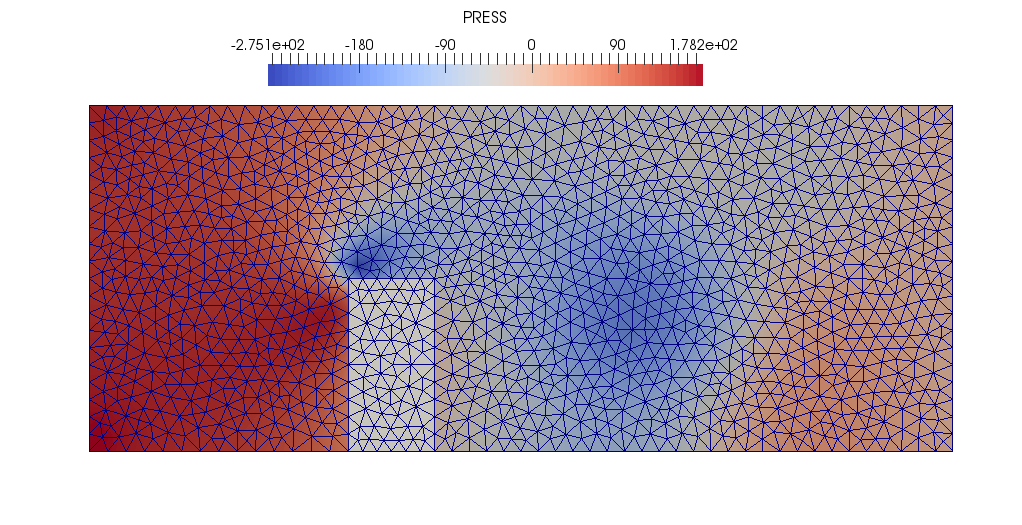
\includegraphics[width=0.5\textwidth]{det_200_firststep}\label{fig:Flap3Det1}}
  \hfill
  \subfloat[Deterministic simulation at time-step 200]{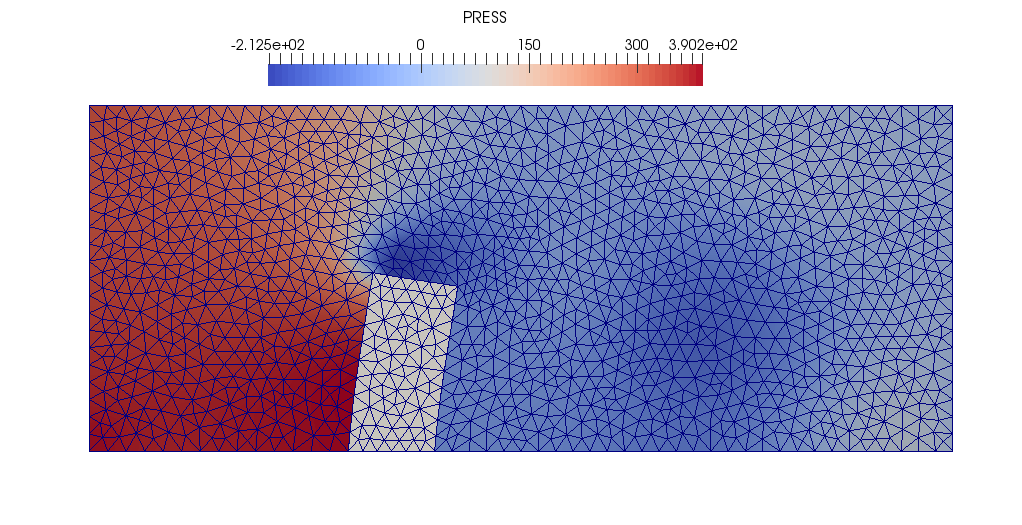
\includegraphics[width=0.5\textwidth]{det_200_laststep}\label{fig:Flap3Det200}}
  \caption{Deterministic simulation of the vertical flap}
  \label{Flap3Det}
  \vspace{-0.4cm}
\end{figure}
The first and the last time step of the deterministic simulation are presented in \refFigure{Flap3Det}, where the visualized fluid's physical parameter was its \emph{pressure}. 

	In the following, the results obtained after the UQ simulations were performed are presented. The next section describes the \emph{one-dimensional} stochastic cases, while the following ones treat \emph{multi-dimensional} scenarios.
\subsection{One Dimensional UQ Simulation}
\label{subsec:1D UQ Simulations}
		
	As the deterministic case was the first important step in the entire set of simulations, the first milestone for the UQ simulations were the \emph{one dimensional} cases. This means that throughout a simulation, \emph{four} out of the \emph{five} input physical parameters are taken to be \emph{sure variables}\footnote{a sure variable is defined to be \emph{exactly determined by given conditions}, i.e. \emph{deterministic}} (see  \cite{Le02} for details), with the fifth being considered to exhibit \emph{uncertainty}. Given the number of input parameters, all five one-dimensional cases were simulated. This means that for the one-dimensional case, an \emph{exhaustive} treatment of uncertainty was made, paving the way for multi-dimensional simulations, as it is explained later in this section. Moreover, for a comprehensive testing and assessment of the employed methods, multiple \emph{configurations} were accounted. First, the variables taken to exhibit uncertainty were modelled as \emph{normal} random variables, and were propagating in the underlying system using both Monte Carlo Sampling and Stochastic Collocations. Afterwards, they were modelled as \emph{uniform} random variables and propagated using Stochastic Collocations. A more detailed presentation is done in the following.
	
	As a starting point, uncertainty is modelled as a \textit{normal random variable} $\Omega$ of the form:
\begin{equation} \label{1DSCGaussian}
\Omega \sim \mathcal{N}(\mu, \sigma^2), \text{with } \sigma = 0.1\mu
\end{equation}
	The first used method was Stochastic Collocations and in order to carry out simulations, the \emph{quadrature degree} (denoted here by \emph{q}) and the \emph{number of coefficients} (denoted here by \emph{n}) have to be established. Based on the maximal implemented q, i.e. ten (c.f. \refSection{sec:Pre-processing}) and the suggested  \emph{rule of thumb} from \cite{Su08}, which states that $q \leq 2 n$, the established combination for this work is \emph{q = 8} and \emph{n = 5}.
\insertfigure{mean_onedim}{Mean for one dimensional scenarios}{fig:SCMeanOnedim}{0.6} % Filename, Caption, Label, Width percent of textwidth
The first processed data sets were the ones corresponding to the \emph{watch point}, which in this case is the upper right corner. Moreover, the quantities of interest were chosen to be the \emph{x axis displacement}, \emph{x axis force} and \emph{y axis force}. 
\insertfigure{var_onedim}{Variance for one dimensional scenarios}{fig:SCVarOnedim}{0.6} % Filename, Caption, Label, Width percent of textwidth 
In \refFigure{fig:SCMeanOnedim} and \refFigure{fig:SCVarOnedim}, the \emph{means} and \emph{variances} of the gathered data are presented, with the means plot including the \emph{deterministic} data as well. From these two plots, several inferences can be made. As a starter, from the first plot, it can be seen that the means of the simulated scenarios almost coincide with each other and even more, are  almost identical to the deterministic data, except for data corresponding to the \emph{Young's modulus}, which, after about time step 80, behaves a little different for the force on the x axis. This outlines two important inferences: first, \emph{on average}, the behaviour is \emph{similar} to the deterministic case and second, \emph{Young's modulus} seems to be the parameter whose uncertainty influences the most the outcomes. Although the plot of the expected values offered the first insights, the \emph{variances} plot is even more interesting, because, among others, it indicates which parameters are important from an uncertain point of view. First of all, it can be seen that, as the variances of the forces exhibit \emph{oscillatory} behaviour, with the one for the y axis force more attenuated, the variance of the x axis displacement increases over time, reaching the peak around time step 190, in the underlying scenario of 200 simulated steps. Moreover, among the five physical parameters, two of them stand out: \emph{fluid's density} and \emph{structure's Young modulus}. From the last observation, it can be pointed out that for the two dimensional case it is expected that combinations including these parameters should have a big impact on the outcomes.

	The results obtained using Stochastic Collocations and normal random variables were compared with the ones output by Monte Carlo Sampling. Considering the high computational and storage demand of this method, a number of \emph{100 samples} were simulated and to quantify the resulting difference, the \emph{mean squared error} (m.s.e.) of the means and variances was computed. 
\begin{table}[h!]
\centering
 \begin{tabular}{|c|c|c|c|} 
 \hline
 statistic & x axis displacement m.s.e. & x axis force m.s.e. & y axis force m.s.e. \\
 \hline 
 mean & 6.238e-10 & 4.974e-4 & 2.737e-4 \\
 \hline 
 variance & 9.603e-14 & 4.359e-4 & 1.436e-4 \\
  \hline
 \end{tabular}
 \caption{Mean squared error for fluid's viscosity}
 \label{table:MCS_SCS_mse}
\end{table}
The comparison was made when the stochastic parameter was \emph{fluid's viscosity}. The statistics plot is outlined in \refFigure{MCS_SCS_com}, whereas the corresponding mean squared errors are presented in \refTable{table:MCS_SCS_mse}.
\begin{figure}[htbp]
  \centering
  \subfloat[Mean comparisson]{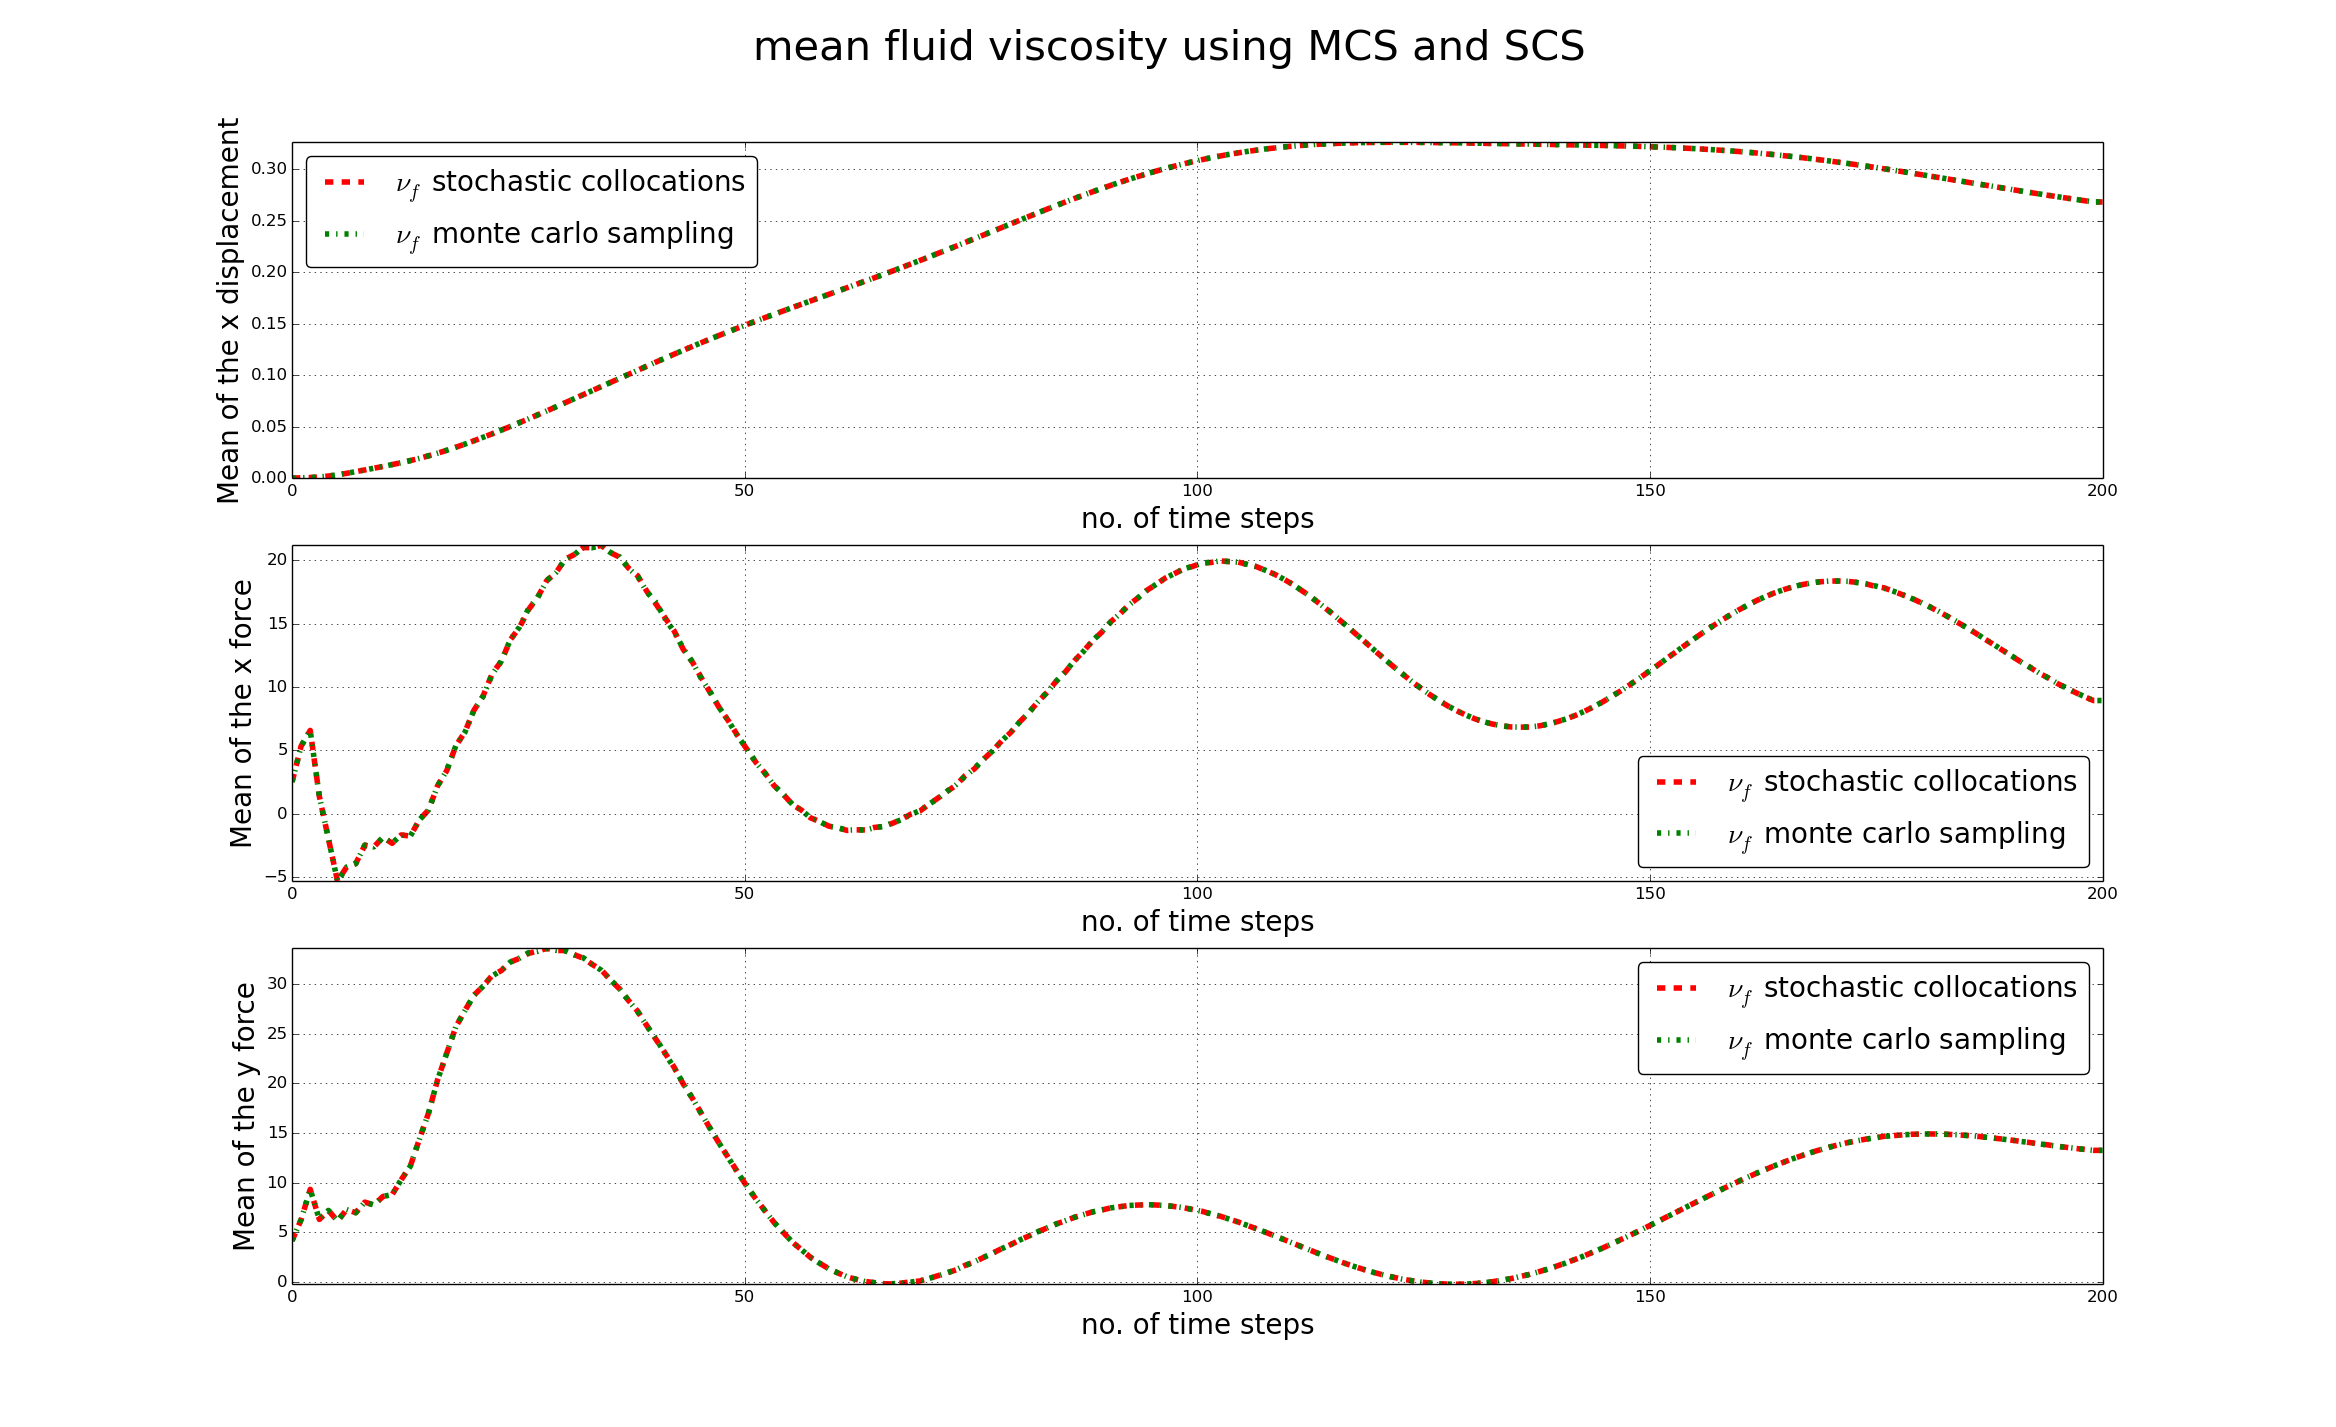
\includegraphics[width=0.5\textwidth]{mean_MCS_SCS_comp}\label{fig:MCS_SCS_mean}}
  \hfill
  \subfloat[Variance comparisson]{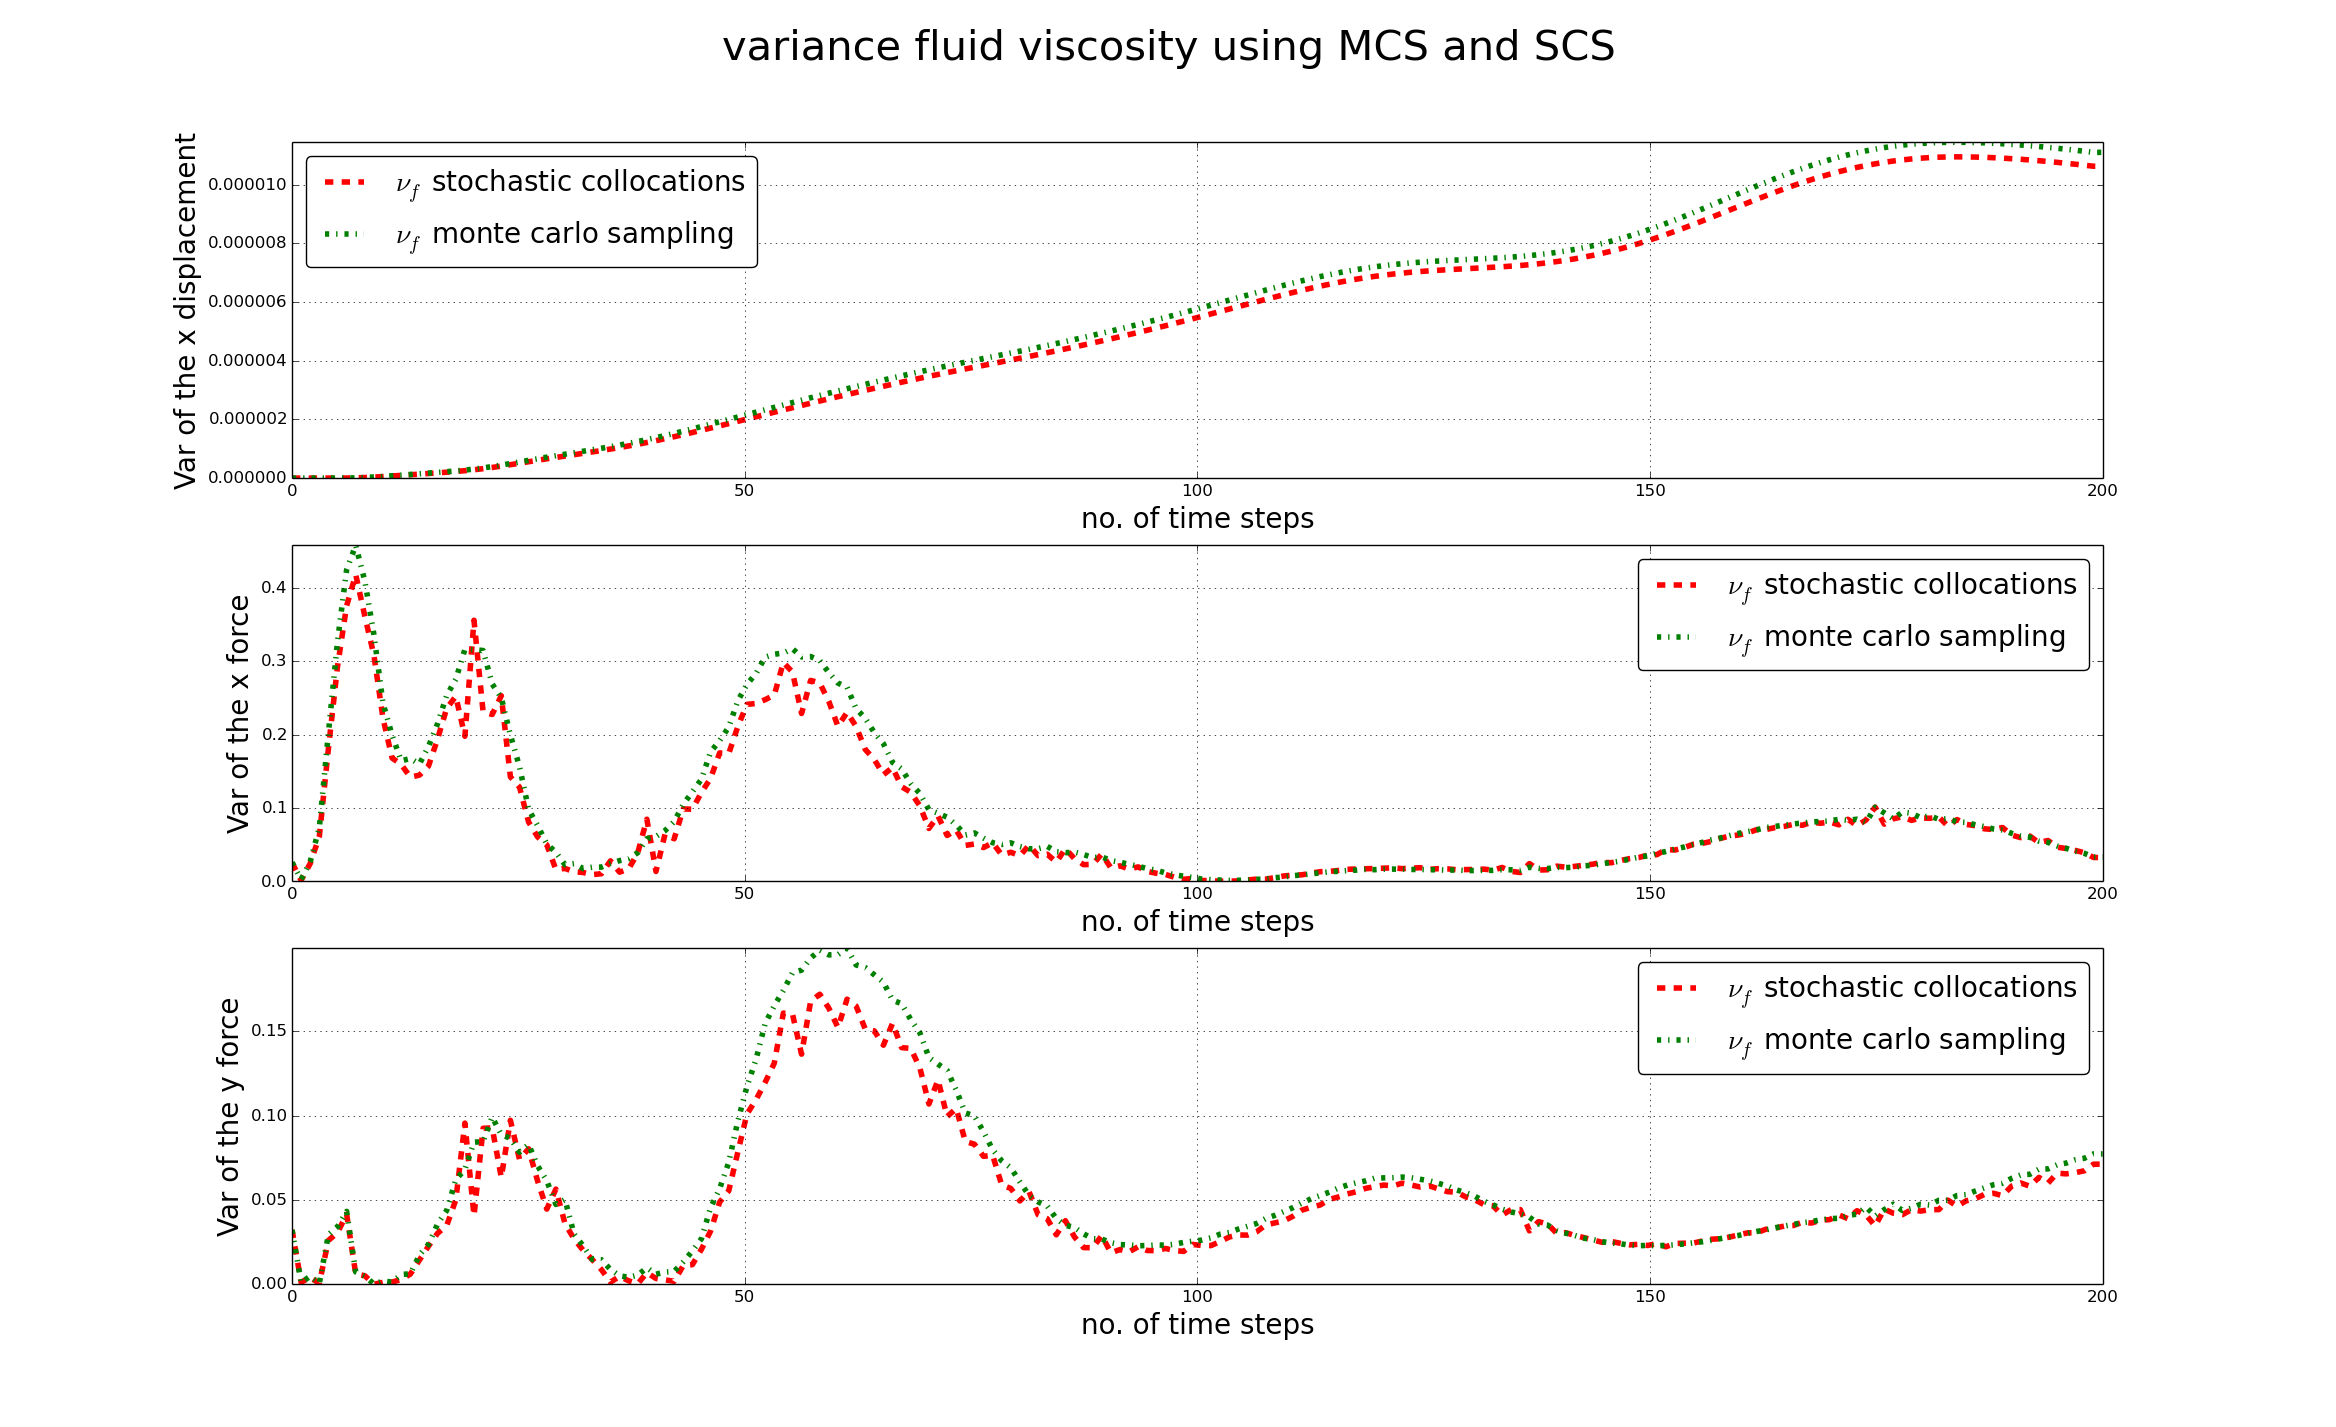
\includegraphics[width=0.5\textwidth]{var_MCS_SCS_comp}\label{fig:MCS_SCS_var}}
  \caption{Comparison of results obtained with both algorithms for fluid's viscosity}
  \label{MCS_SCS_com}
  \vspace{-0.4cm}
\end{figure}
Based on these results, it results that Stochastic Collocations with a quadrature degree of order 8 and 5 expansion coefficients converges. Moreover, similar results were obtained when testing for the other four parameters and hence, ascertaining the previous assertion.

	The next step was to get a better understanding of how the normal distribution affects the outcomes. To this extent, based on \refEquation{1DSCGaussian}, the uncertain parameters were modelled as \emph{uniform random variables} $\Gamma$ of the form:
\begin{equation} \label{1DSCUniform}
\Gamma \sim \mathcal{U}(a, b), \text{with } a = 0.9\mu \text{ and } b = 1.1\mu, 
\end{equation}
where $\mu$	is the mean used for normal random variables. As with Monte Carlo Sampling, the comparison was made when the stochastic parameter was \emph{fluid's viscosity}. The statistics plot is outlined in \refFigure{SCS_com} and the corresponding mean squared errors are presented in \refTable{table:SCS_nor_uni_mse}.
\begin{table}[h!]
\centering
 \begin{tabular}{|c|c|c|c|} 
 \hline
 statistic & x axis displacement m.s.e. & x axis force m.s.e. & y axis force m.s.e. \\
 \hline 
 mean & 1.049e-8 & 9.987-4 & 5.072e-4 \\
 \hline 
 variance & 1.244e-14 & 4.737e-4 & 1.568e-4 \\
  \hline
 \end{tabular}
 \caption{Mean squared error for fluid's viscosity}
 \label{table:SCS_nor_uni_mse}
\end{table}
\begin{figure}[htbp]
  \centering
  \subfloat[Mean comparisson]{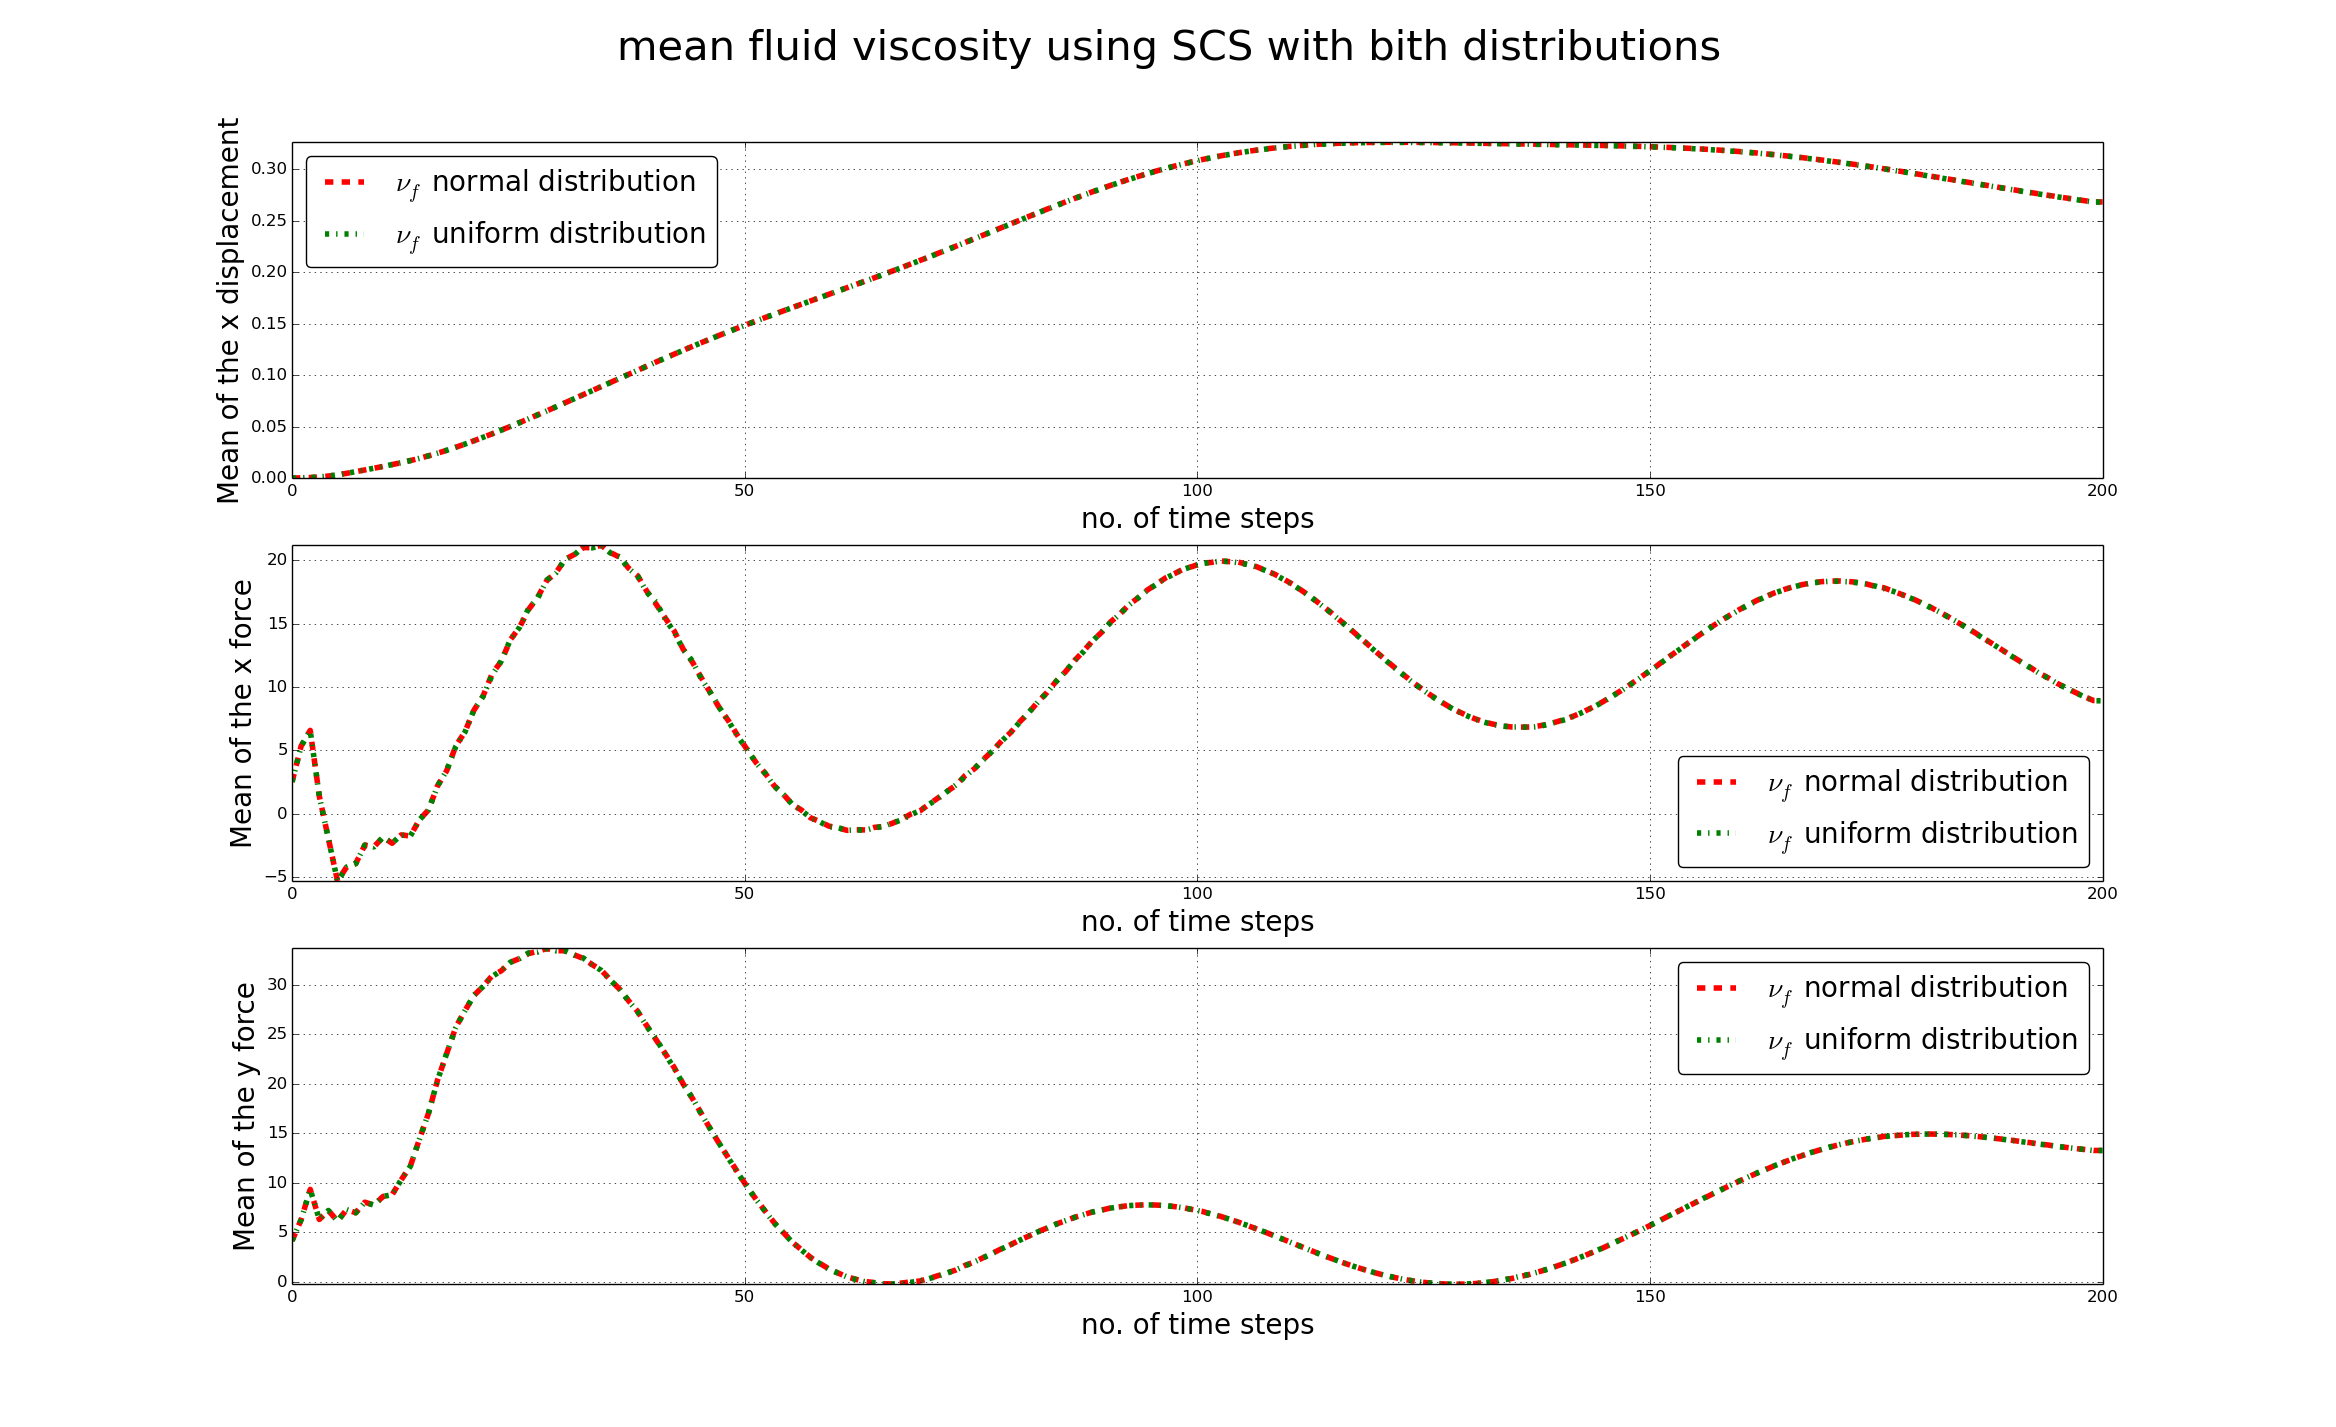
\includegraphics[width=0.5\textwidth]{mean_SCS_comp}\label{fig:SCS_nor_uni_mean}}
  \hfill
  \subfloat[Variance comparisson]{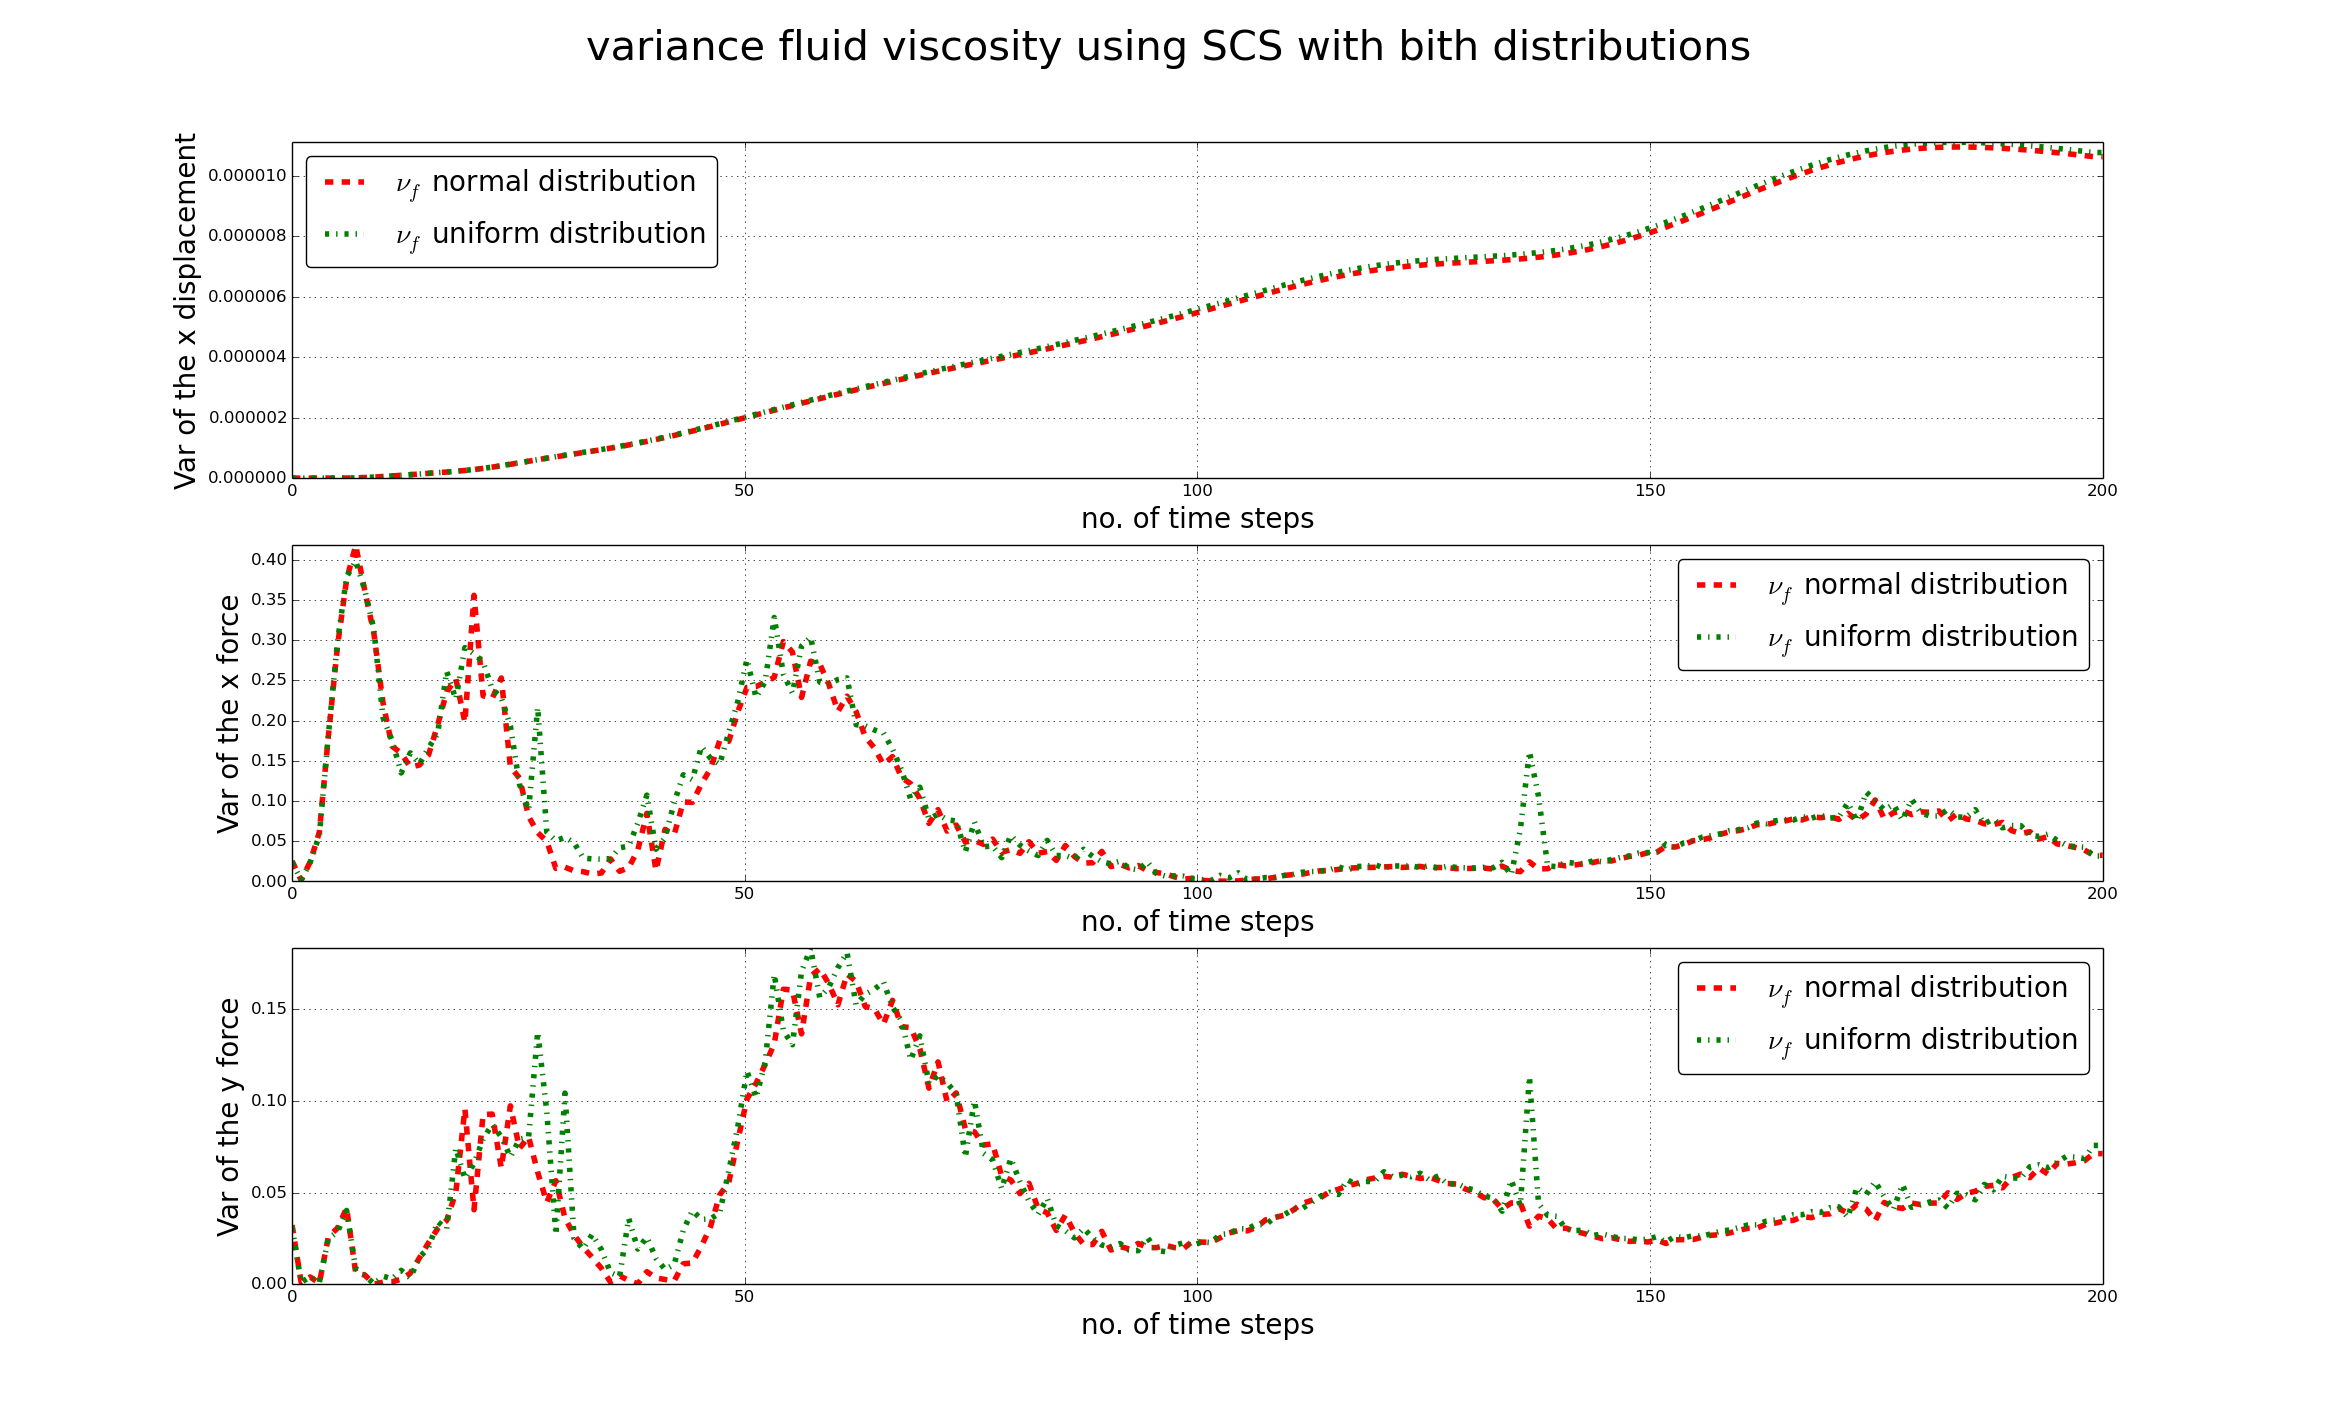
\includegraphics[width=0.5\textwidth]{var_SCS_comp}\label{fig:SCS_nor_uni_var}}
  \caption{Comparison of results obtained with normal and uniform for fluid's viscosity}
  \label{SCS_com}
  \vspace{-0.4cm}
\end{figure}
Likewise Monte Carlo Sampling, the results obtained by using uniform random variables were very similar to the case when using normal random variables. Even more, similar results were obtained for the other four parameters as well. 

	Based on these results, it follows that Stochastic Collocations with normal random variables as in \refEquation{1DSCGaussian}, is enough for performing uncertainty propagation in the underlying scenario. That is why, in the following, only results outlined by this strategy are presented. 
\subsection{Two Dimensional UQ Simulations}
\label{subsec:2D UQ Simulations}

\subsection{Five Dimensional UQ Simulations}
\label{5D UQ Simulations}

\section{Scenario II - rename}
\label{Scenario II}




		% ---------------------------------------------------------------------------
		%
		% Discussion and outlook
		%
		% ---------------------------------------------------------------------------
		\chapter{Conclusions}
\label{chapter:Conclusions}
 
\section{Summary}
\label{sec:Summary}
\begin{itemize}
\item
\end{itemize}	
\section{Outlook}
\label{sec:Outlook}
\begin{itemize}
\item
\end{itemize}	


		
		
		% ---------------------------------------------------------------------------
		%
		% Appendix
		%
		% ---------------------------------------------------------------------------
		
		\part*{Appendix}
		\addcontentsline{toc}{part}{Appendix}
		
		\appendix %---------------------------------------
		
		\chapter{To be written}
%\section{Detailed Validation Results}
\label{chapter:To be written}
		

  \clearemptydoublepage
  
	\bibliography{bibliography/literature}
	
 
\end{document}

